\chapter{Results and Conclusion} \label{ch:cando}

Up to this point I have given an overview of the physics background for jets created in igh energy particle collisions, the ALICE detector, and the steps needed to prepare the data for an analyisis.  The final portion of this thesis will put all of the results and corrections together and present the final cross sections and the comparison to different theoretical models.  However, In order to present the final cross-section we will discuss the systematic errors that contribute to the final uncertainty in my reported results.

\section{Systematic Uncertainties}

Systematic uncertainties arise due to our limited knowledge of the precise operating conditions and performance of the experiment and also due to any bias in our understanding of how to fundamental model the interactions.  They systematics may therefore be broken into two components: uncertainties to the jet energy scale (JES) which shifts the momentum spectra along the x-axis and uncertainties in the jet yield which shift the spectra along the y-axis.  The systematical and statistical uncertainties presented in this analysis will be presented as errors to the yield of the spectra.  Due to the fact that the $p_{T}$ distribution follows a power law function, $dN/dp_{T} \sim p_{T}^{-5}$ uncertainties in the JES are converted to yield uncertainties by dividing each one by 5.
Due to the low statistics at the highest $p_{T}$ bins in this analysis, uncertainties in this regime my have large statistical fluctuations.  Small ,systematic variations for the input of the jet spectra will have a dramatic effect over sparsely filled bins versus bins with a low granularity.  As such it may be necessary to extrapolate the systematic from a low $p_{T}$ bin to those at the highest $p_{T}$ range.  The systematic were performed on both the MB and EMCal triggered data samples but no large variation was observed between the two, thus only the uncertainties from the MB sample are shown and are extrapolated to the triggered data.


\subsection{Systematic Uncertainty to Jet Energy Scale}

The following sections present and discuss the uncertainties caused by shifts to the JES.

\subsubsection{Tracking Efficiency Sensitivity}
Only a fraction of charged tracks generated by the hard scattering of two protons will be detected in the TPC due to finite track efficiency.  Uncertainties in the efficency of the TPC were studied and found to account for a 5\% discrepancy\cite{Abelev:2013ala}.  Reproducing this efficency was performed by randomly throwing out 5\% of the tracks from each event from the 8 TeV data samples and remeasuring the jet spectra.  All of the inputs for jet finding were maintained.


\begin{figure*}[t!]
$\begin{array}{rl}
    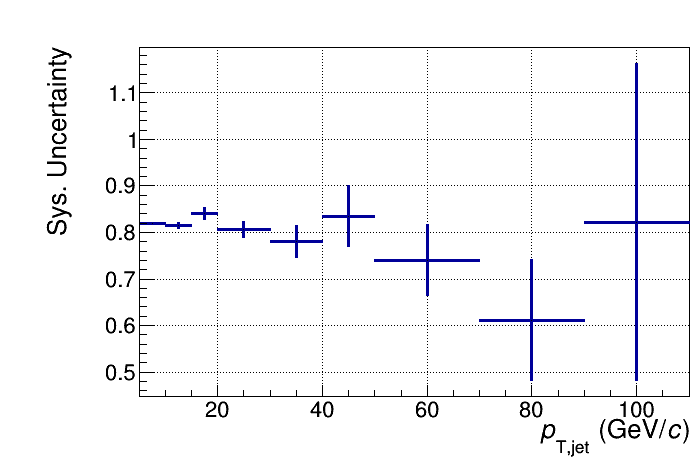
\includegraphics[width=0.40\textwidth]{SysR02_TrkEff} &
    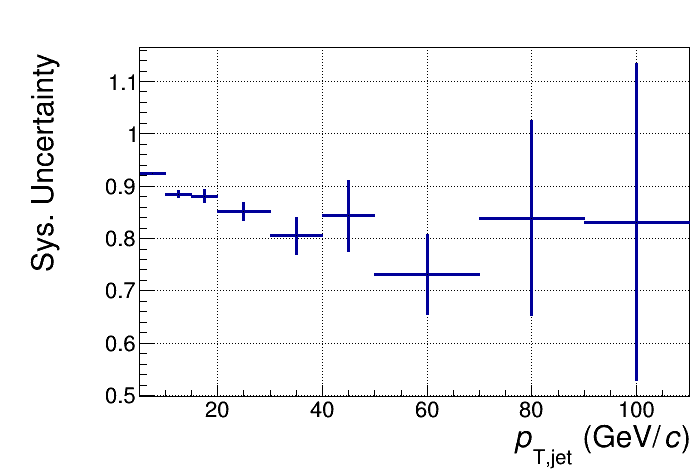
\includegraphics[width=0.40\textwidth]{SysR03_TrkEff}\\
    \multicolumn{2}{c}{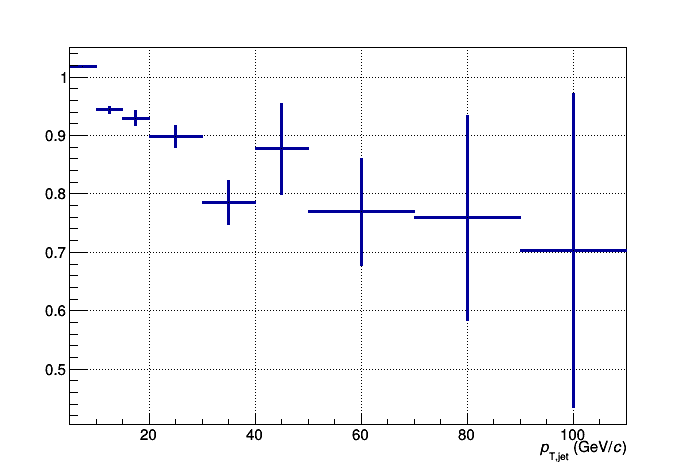
\includegraphics[width=0.40\textwidth]{SysR04_TrkEff}}
\end{array}$
\caption[Systematic due to TPC tracking efficiency.]{\label{fig:trkeff}Systematic due to TPC tracking efficiency; R = 0.2 \textit{(top left)}, R = 0.3 \textit{(top right)}, R = 0.4 \textit{(bottom)}.}
\end{figure*}

\noindent
Figure \ref{fig:trkeff} shows the systematical uncertainties for R = 0.2 (top left), R = 0.3 (top right), and R = 0.4 (bottom) jets.  A 10\% systematic was applied to R = 0.2 and R = 0.3 jets while a 15\% systematic uncertainty was given to R = 0.4 jets for this analysis.

\subsubsection{Hadronic Correction Systematic}

\begin{figure*}[t!]
$\begin{array}{rl}
    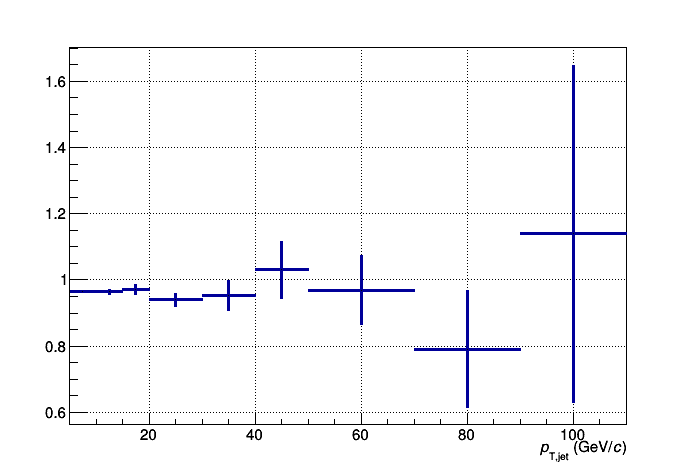
\includegraphics[width=0.40\textwidth]{SysR02_F07} &
    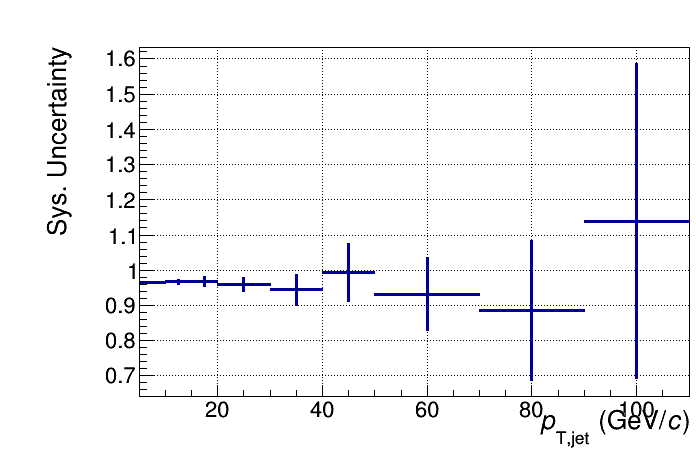
\includegraphics[width=0.40\textwidth]{SysR03_F07}\\
    \multicolumn{2}{c}{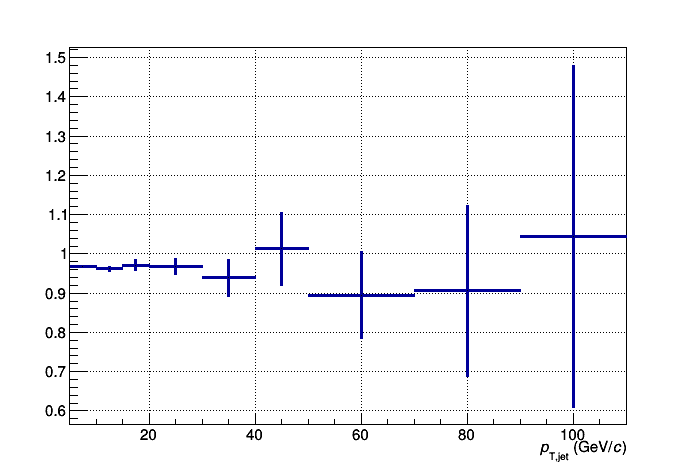
\includegraphics[width=0.40\textwidth]{SysR04_F07}}
\end{array}$
\caption[Systematic due to Hadronic correction.]{\label{fig:hadeff}Systematic due to hadronic correction efficiency; R = 0.2 \textit{(top left)}, R = 0.3 \textit{(top right)}, R = 0.4 \textit{(bottom)}.}
\end{figure*}

\subsubsection{Sensativity to EMCal Clusterization Algorithm}
As previously stated, the clusterizer used in this thesis was the v2 algorithm. This algorithm was used in both the detector-level Monte Carlo and data analysis.  In order to test the sensitivity the JES has to the clusterization algorithm a different algorithm was chosen and a new spectra was generated.  The v1 algorithm was choosen and is similar to the v2 algorithm with the exception that the total size of the cluster is forced to be smaller then nine towers.  Similar to the other systematic presented we see a large anti-correlated bin-to-bin variatiaions at high-$p_{T}$ due to sparsely field binning.  

\begin{figure*}[t!]
$\begin{array}{rl}
    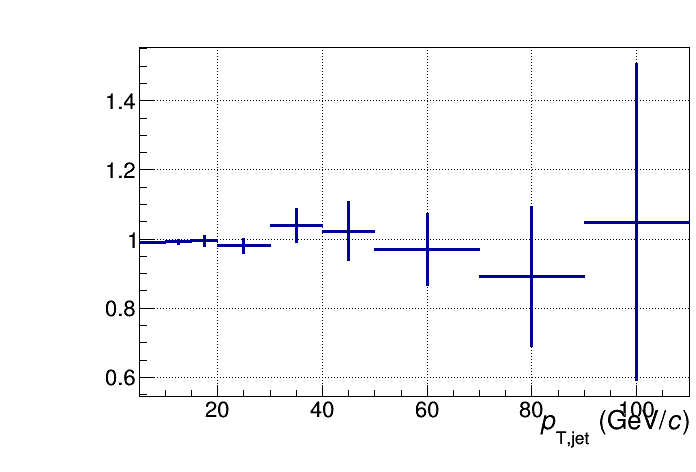
\includegraphics[width=0.40\textwidth]{SysR02_v1Clusterization} &
    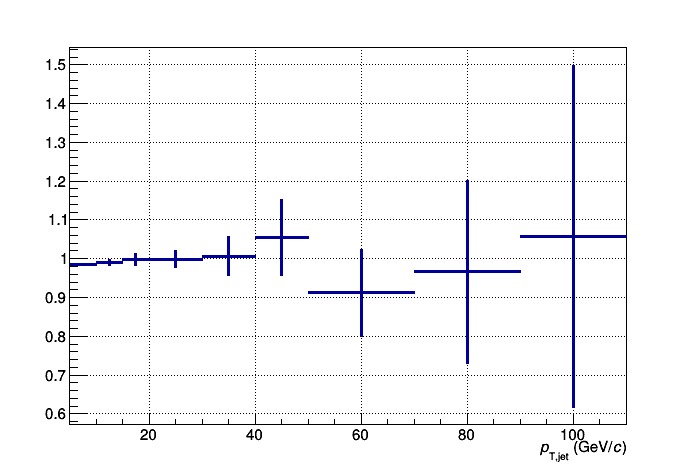
\includegraphics[width=0.40\textwidth]{SysR03_v1Clusterization}\\
    \multicolumn{2}{c}{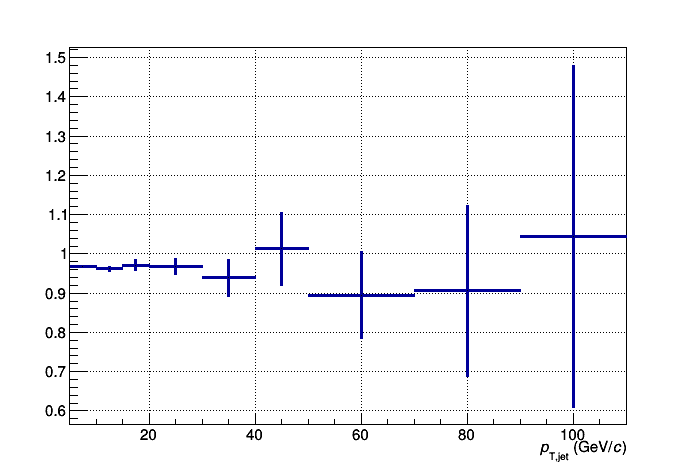
\includegraphics[width=0.40\textwidth]{SysR04_F07}}
\end{array}$
\caption[Systematic due to clusterization algorithm.]{\label{fig:cluseff}Systematic due to EMCal clusterization algorithm; R = 0.2 \textit{(top left)}, R = 0.3 \textit{(top right)}, R = 0.4 \textit{(bottom)}.}
\end{figure*}

\subsection{Systematic Uncertainty to Jet Yield}
The following sections discuss the systematic uncertainties affecting the jet yield.

\subsubsection{Track $p_{T}$ resolution}
The momentum resolution of TPC is estimated using the covariance matrix, Figure\ref{fig:trackpcovmatrix}, generated from a Kalman filtering\cite{Fruhwirth:1987fm} pad signal on the TPC read-out region.  To estimate the systematic due to the $p_{T}$ resolution tracks are smeared 

\begin{figure}[h]
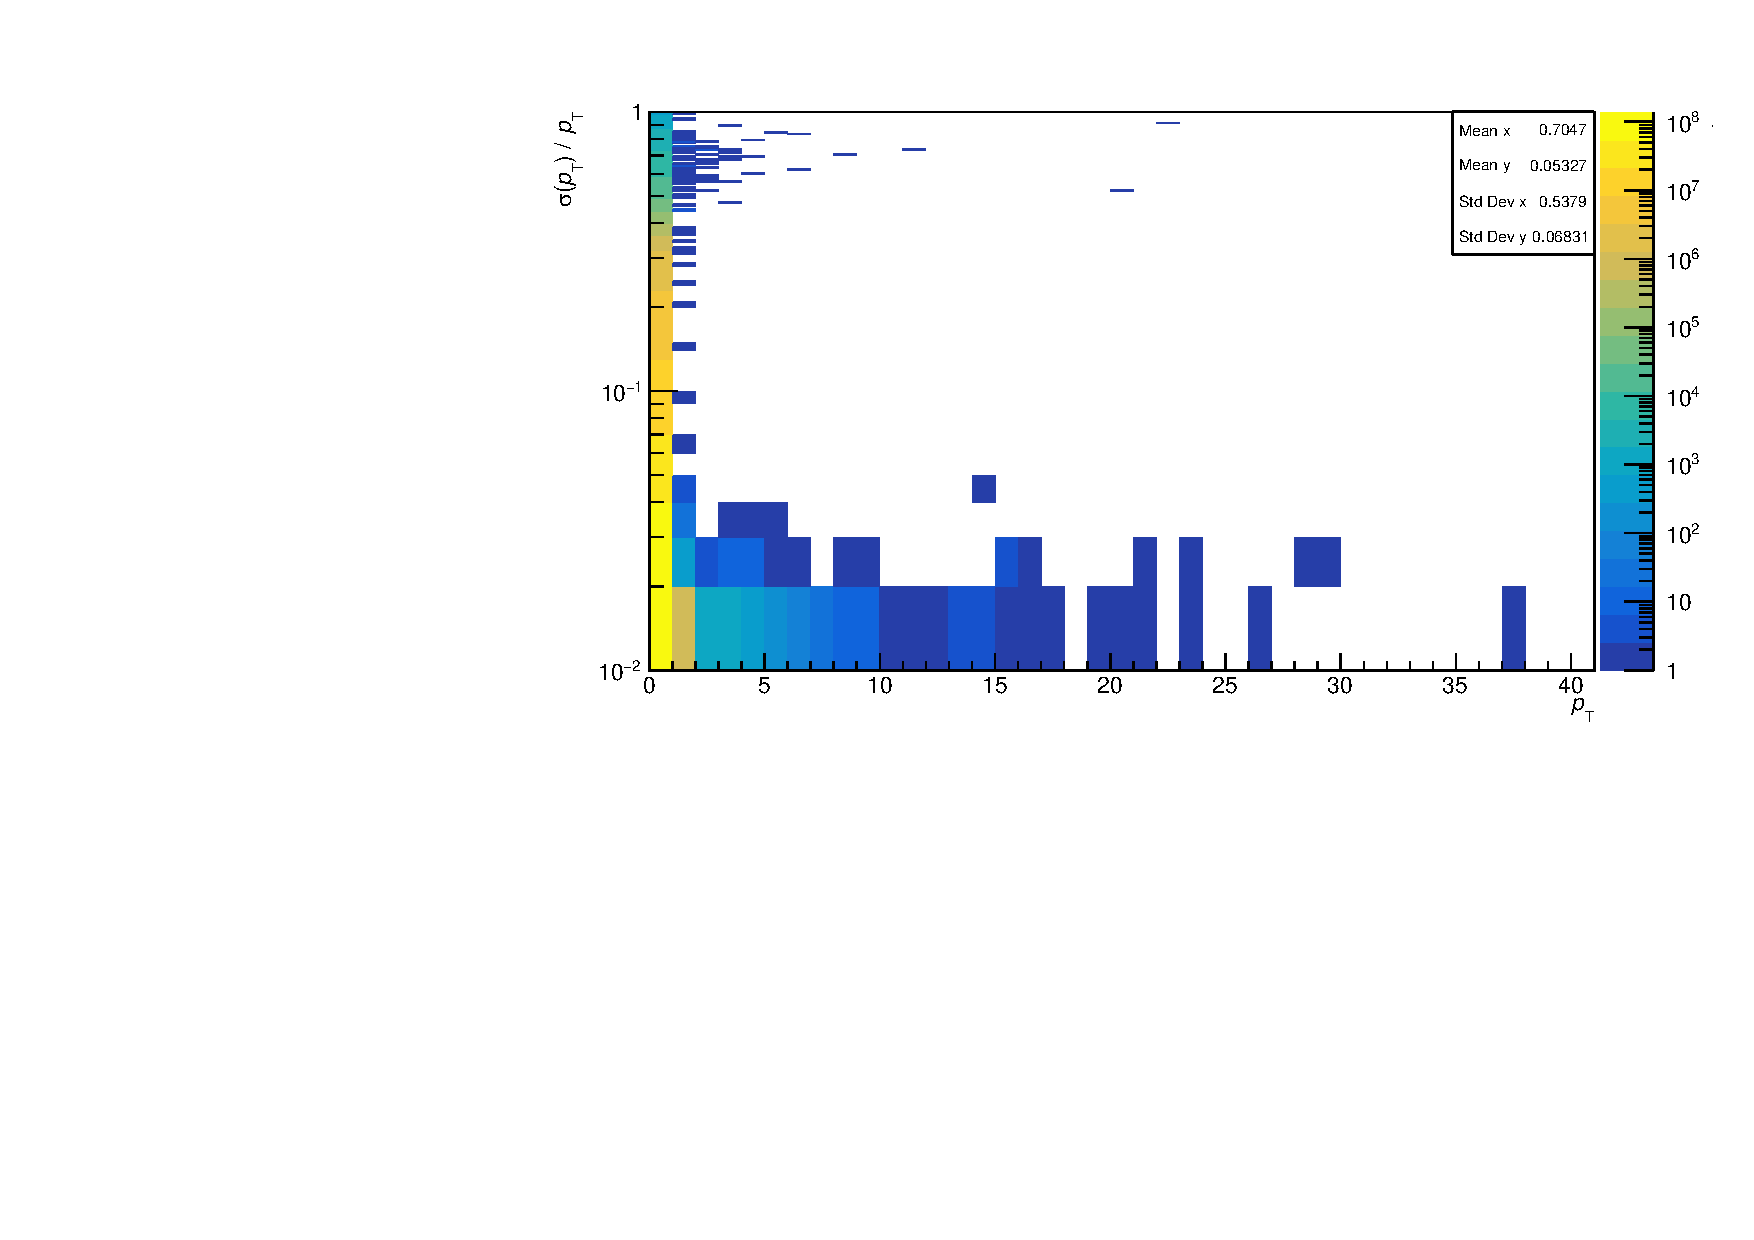
\includegraphics[width=8cm]{trackcovmatrix}
\centering
\caption{Inclusive track resolution, Min Bias 8 TeV.}
\label{fig:trackpcovmatrix}
\end{figure}

Most tracks have below 1\% momentum resolution and the tracks with $\sigma(p_{T})/p_{T} \geq$ 1\% tend to be tracks below 200 MeV tracks.  To measure the $p_{T}$ resolution I smeared each track from the Min Bias data by a Gaussian function which would alter the track $p_{T}$ by up to 1\% of its original value and remeasure the spectra.  

\begin{figure*}[t!]
$\begin{array}{rl}
    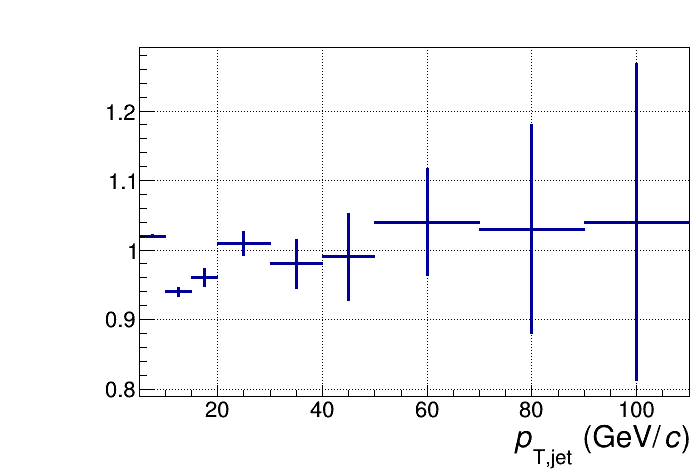
\includegraphics[width=0.40\textwidth]{SysR02_PtReso} &
    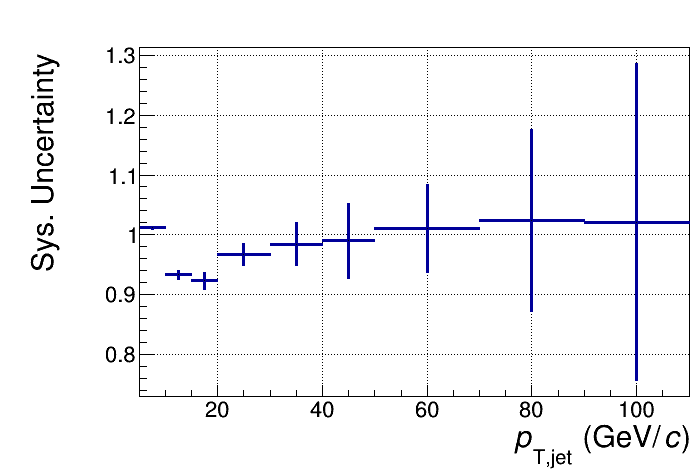
\includegraphics[width=0.40\textwidth]{SysR03_PtReso}\\
    \multicolumn{2}{c}{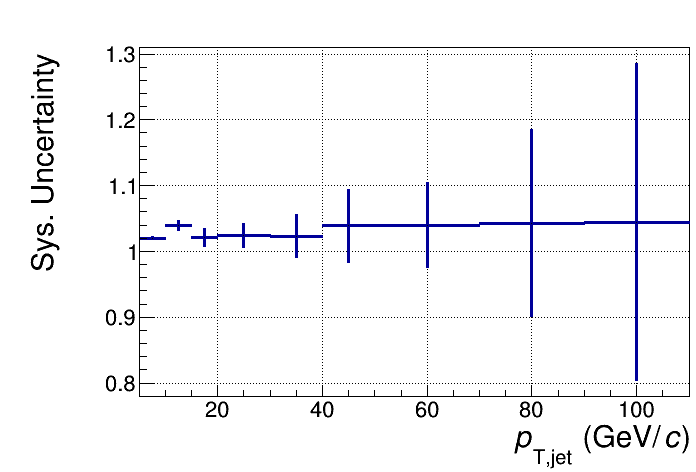
\includegraphics[width=0.40\textwidth]{SysR04_PtReso}}
\end{array}$
\caption[Systematic due to $P_{T}$ resolution.]{\label{fig:pTeff}$P_{T}$ resolution; R = 0.2 \textit{(top left)}, R = 0.3 \textit{(top right)}, R = 0.4 \textit{(bottom)}.}
\end{figure*}


\subsubsection{Cluster Energy resolution}

\begin{figure*}[t!]
$\begin{array}{rl}
    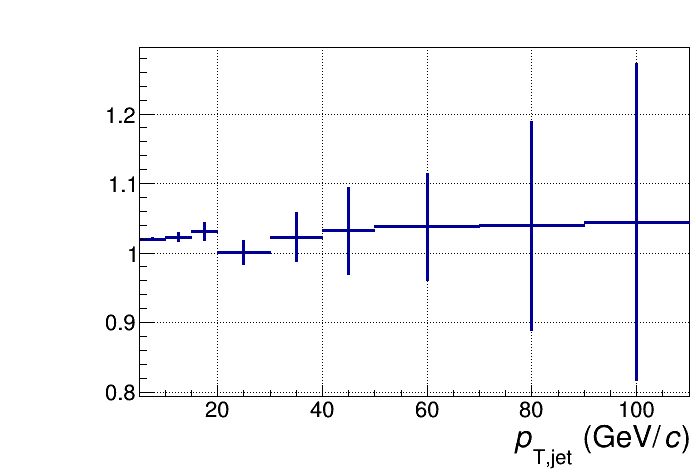
\includegraphics[width=0.40\textwidth]{SysR02_EReso} &
    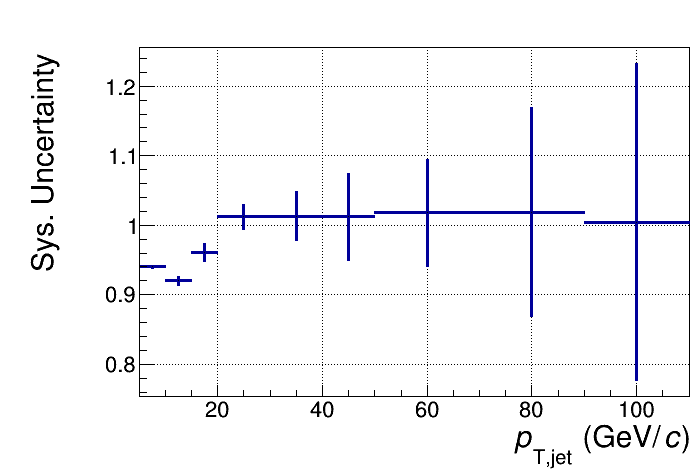
\includegraphics[width=0.40\textwidth]{SysR03_EReso}\\
    \multicolumn{2}{c}{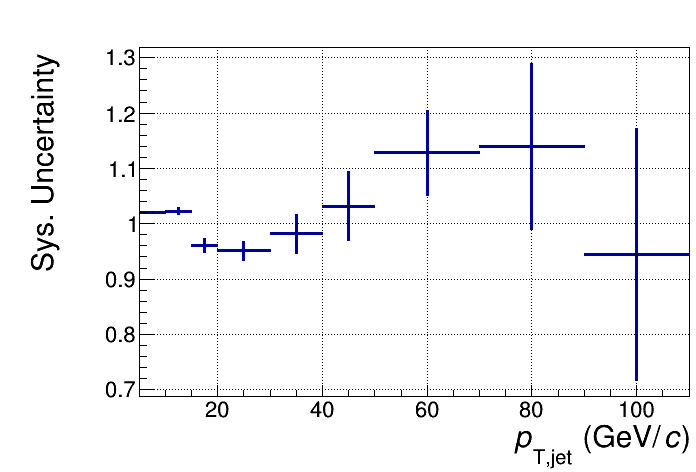
\includegraphics[width=0.40\textwidth]{SysR04_EReso}}
\end{array}$
\caption[Systematic due to energy resolution.]{\label{fig:pTeff}energy resolution; R = 0.2 \textit{(top left)}, R = 0.3 \textit{(top right)}, R = 0.4 \textit{(bottom)}.}
\end{figure*}

\subsubsection{Luminosity and Uncertainty}

The luminosity of a hadronic collider, $\mathscr{L}$, is given by the expression



\begin{equation}
\mathscr{L} = \frac{R}{\sigma}
\label{eq:xlumdef}
\end{equation}

\noindent
where R is the interaction rate and $\sigma$ is the visible cross section.  Due to the fact that we only measure events within a 10 cm window within the primary vertex region we must scale the total luminosity to that which is delievered within the primary vertex region of the ALICE experiment.  This scale factor is determined by dividing the total number of MB events to those accepted within the 10 cm window.  $N^{tot}_{MB} / N^{10 cm vertex}_{MB}$ = 1.024 from the acceptance criteria held in this analysis.
The luminosity along with its uncertainty were determined during a a special Van der Meer scan run in April of 2012\cite{ALICE-PUBLIC-2017-002}.  The total systematic uncertainty for the minimum bias (MB) trigger were obtained by measuring the visible cross section using the T0 and V0 detectors.  The MB trigger was defined as V0AND which required a hit in both the V0A and V0C.  The cross section was reported as being a combined average for MB with the V0AND as, 

\begin{equation}
\sigma_{V0} = (55.8 \pm 1.2) mb
\label{eq:xlumdef}
\end{equation}

\noindent
with a combined systematic uncertainty of 2.19\% on the visible cross section and 2.60\% on the luminosity. 


\subsubsection{Total Uncertainty}

A summary of the total systematic errors used in the final analysis.

\begin{tabular}{ |p{5cm}||p{3cm}|p{3cm}|p{3cm}|  }
 \hline
 \multicolumn{4}{|c|}{Systematic Errors} \\
 \hline
 Systematic &R = 0.2 Jets & R = 0.3 Jets& R = 0.4 Jets\\
 \hline
Clusterization (low-$p_{T}$) & 1.0\%    &1.0\%&  3.0\%\\
 (high-$p_{T}$)           &  5.0\%  & 10.0\%   &  10.0\%\\
Hadronic (all bins)&   5.0\% & 4.0\% & 5.0\%\\
Track Eff (low-$p_{T}$)&20.0\% & 15.0\% & 15.0\%\\
 (high-$p_{T}$)            &  25.0\%  & 20.0\%   &  25.0\%\\
Unfolding (all bins)& 6.0\% & 6.0\%&  6.0\%\\
$p_{T}$ Resolution & 2.0\% & 1.0\% & 4.0\%\\
E Resolution& 2.0\%   &1.0\% & 5.0\%\\
Luminosity (all bins) & 2.2\%  & 2.2 \% & 2.2\%\\
 \hline
 \hline
Total Sys (low-$p_{T}$) & 8.9\%  & 6.6\% & 10.9\%\\
(high-$p_{T}$) & 10.3\%  & 9.1 \% & 14.5\%\\
\hline
\end{tabular}

\
\newline
The systematics from the yield and JES are added in quadrater together to form the final reported total systematic errors per given $p_{T}$ bin.
\newpage

\section{8 TeV Inclusive Jet Results and Discussion}

\subsubsection{Differential Jet Cross-Section}

\begin{figure}[h]
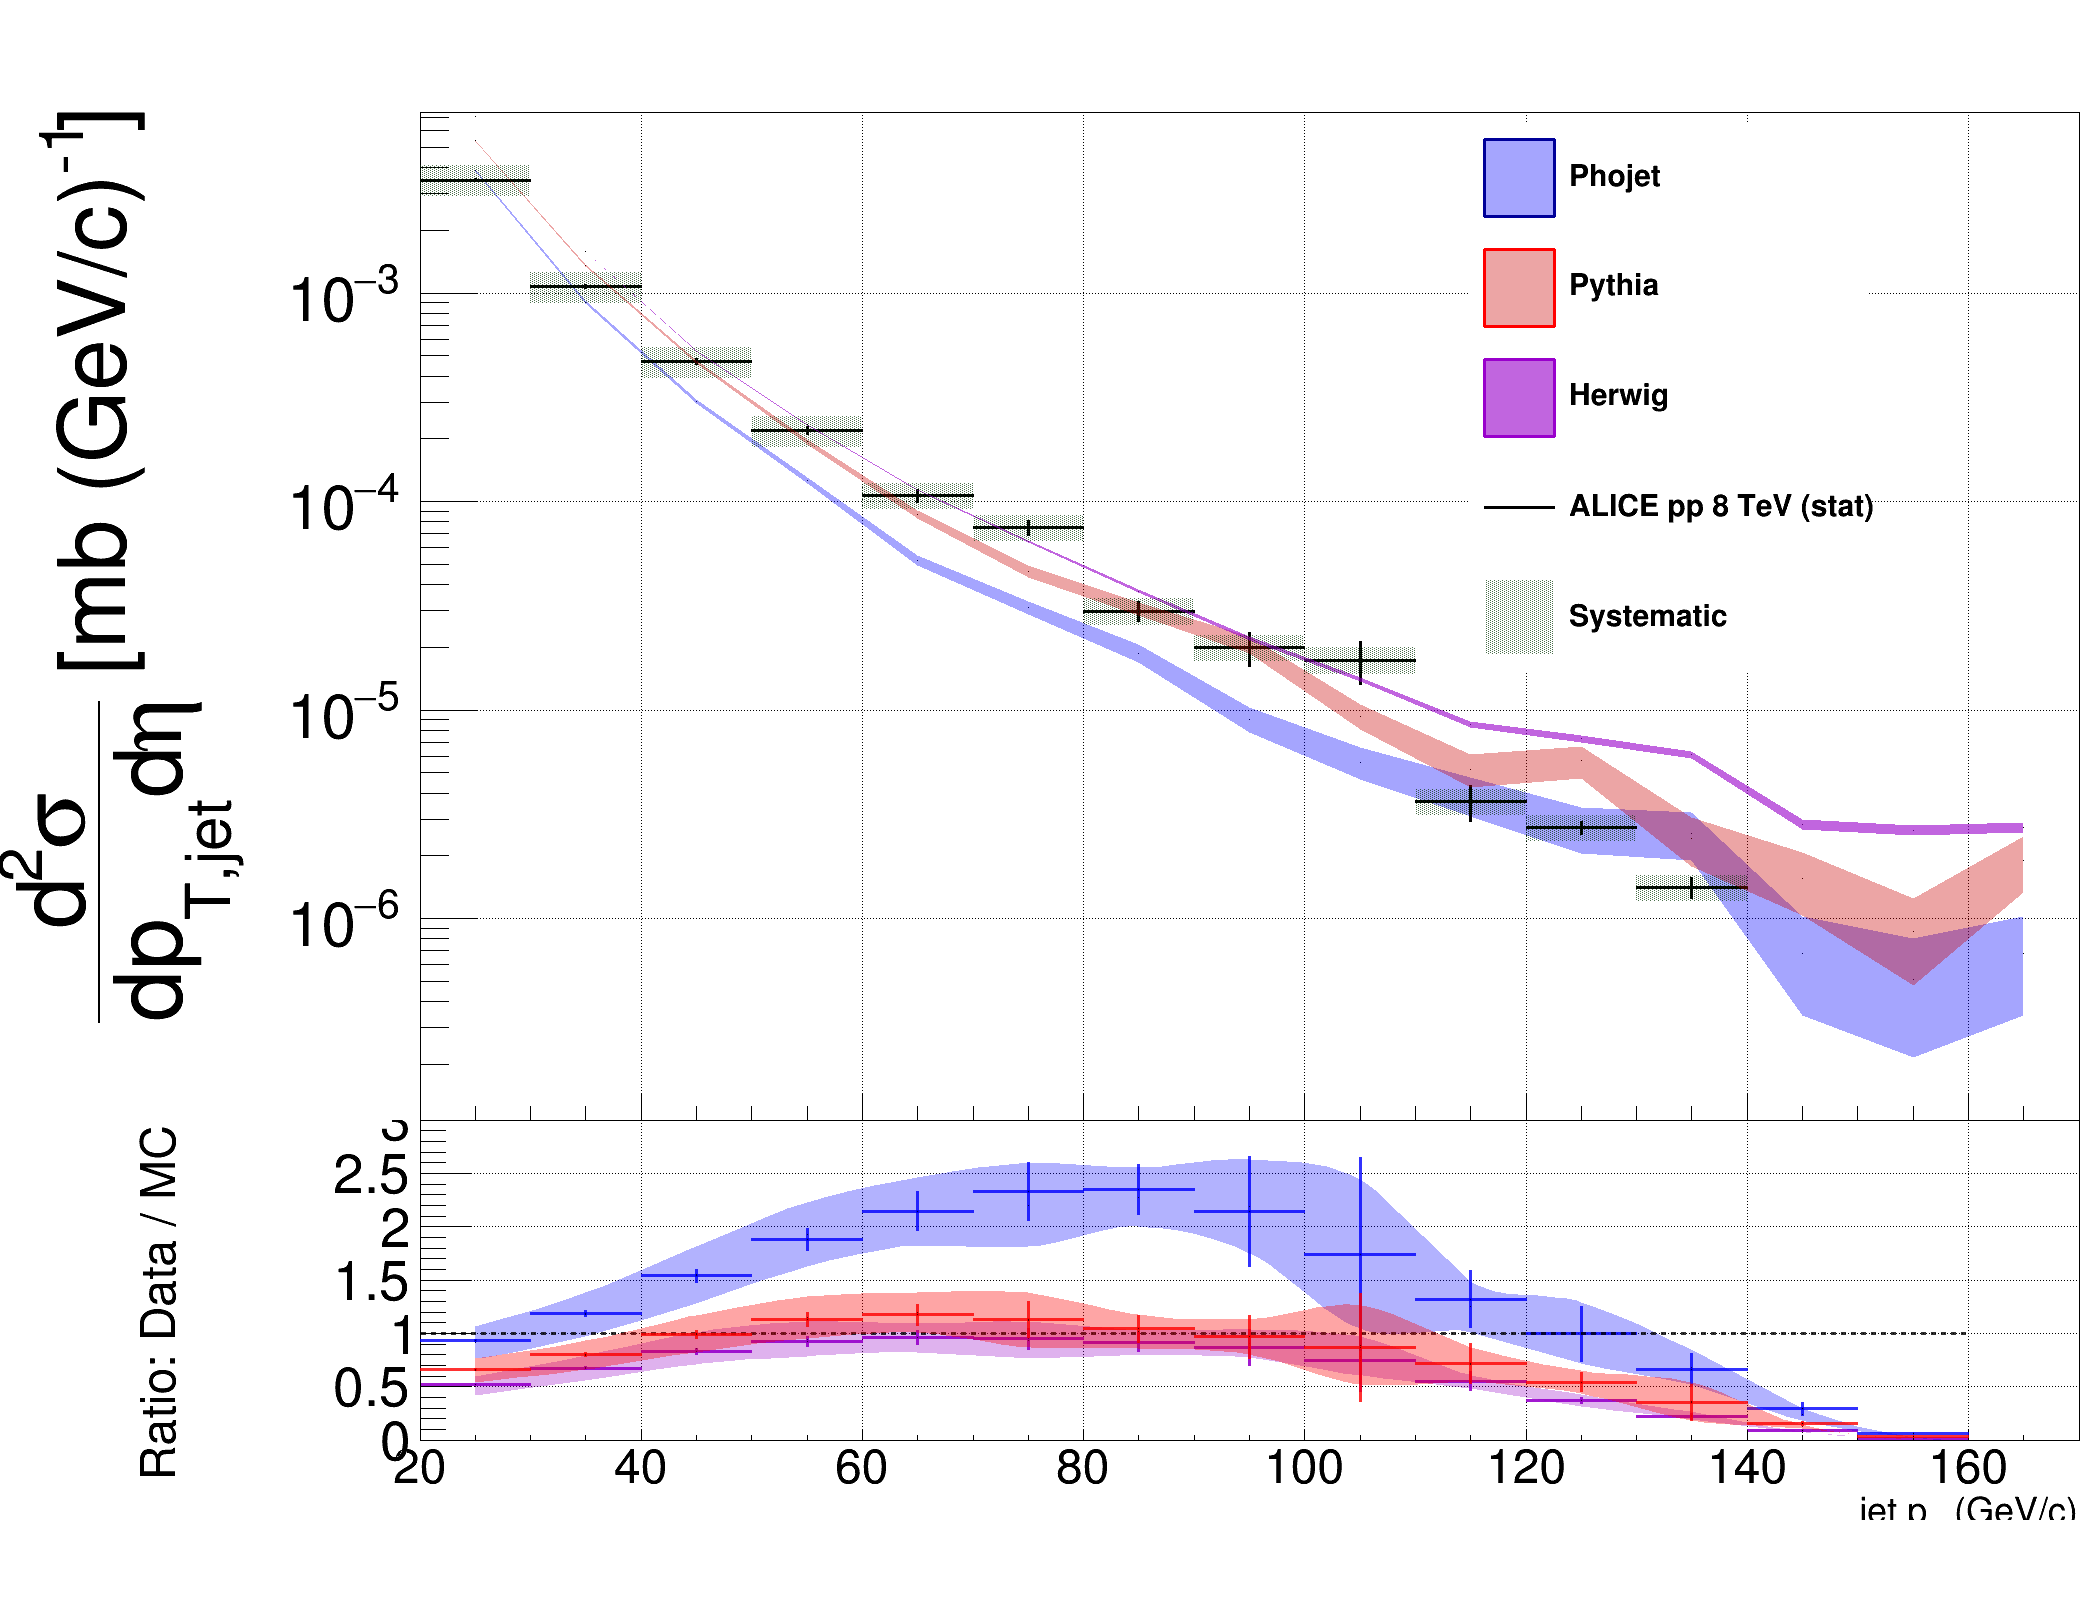
\includegraphics[width=8.5cm]{XSecR02}
\centering
\caption{8 TeV inclusive jet differential cross-section for R = 0.2.}
\label{fig:JetXsecR02}
\end{figure}

\begin{figure}[h]
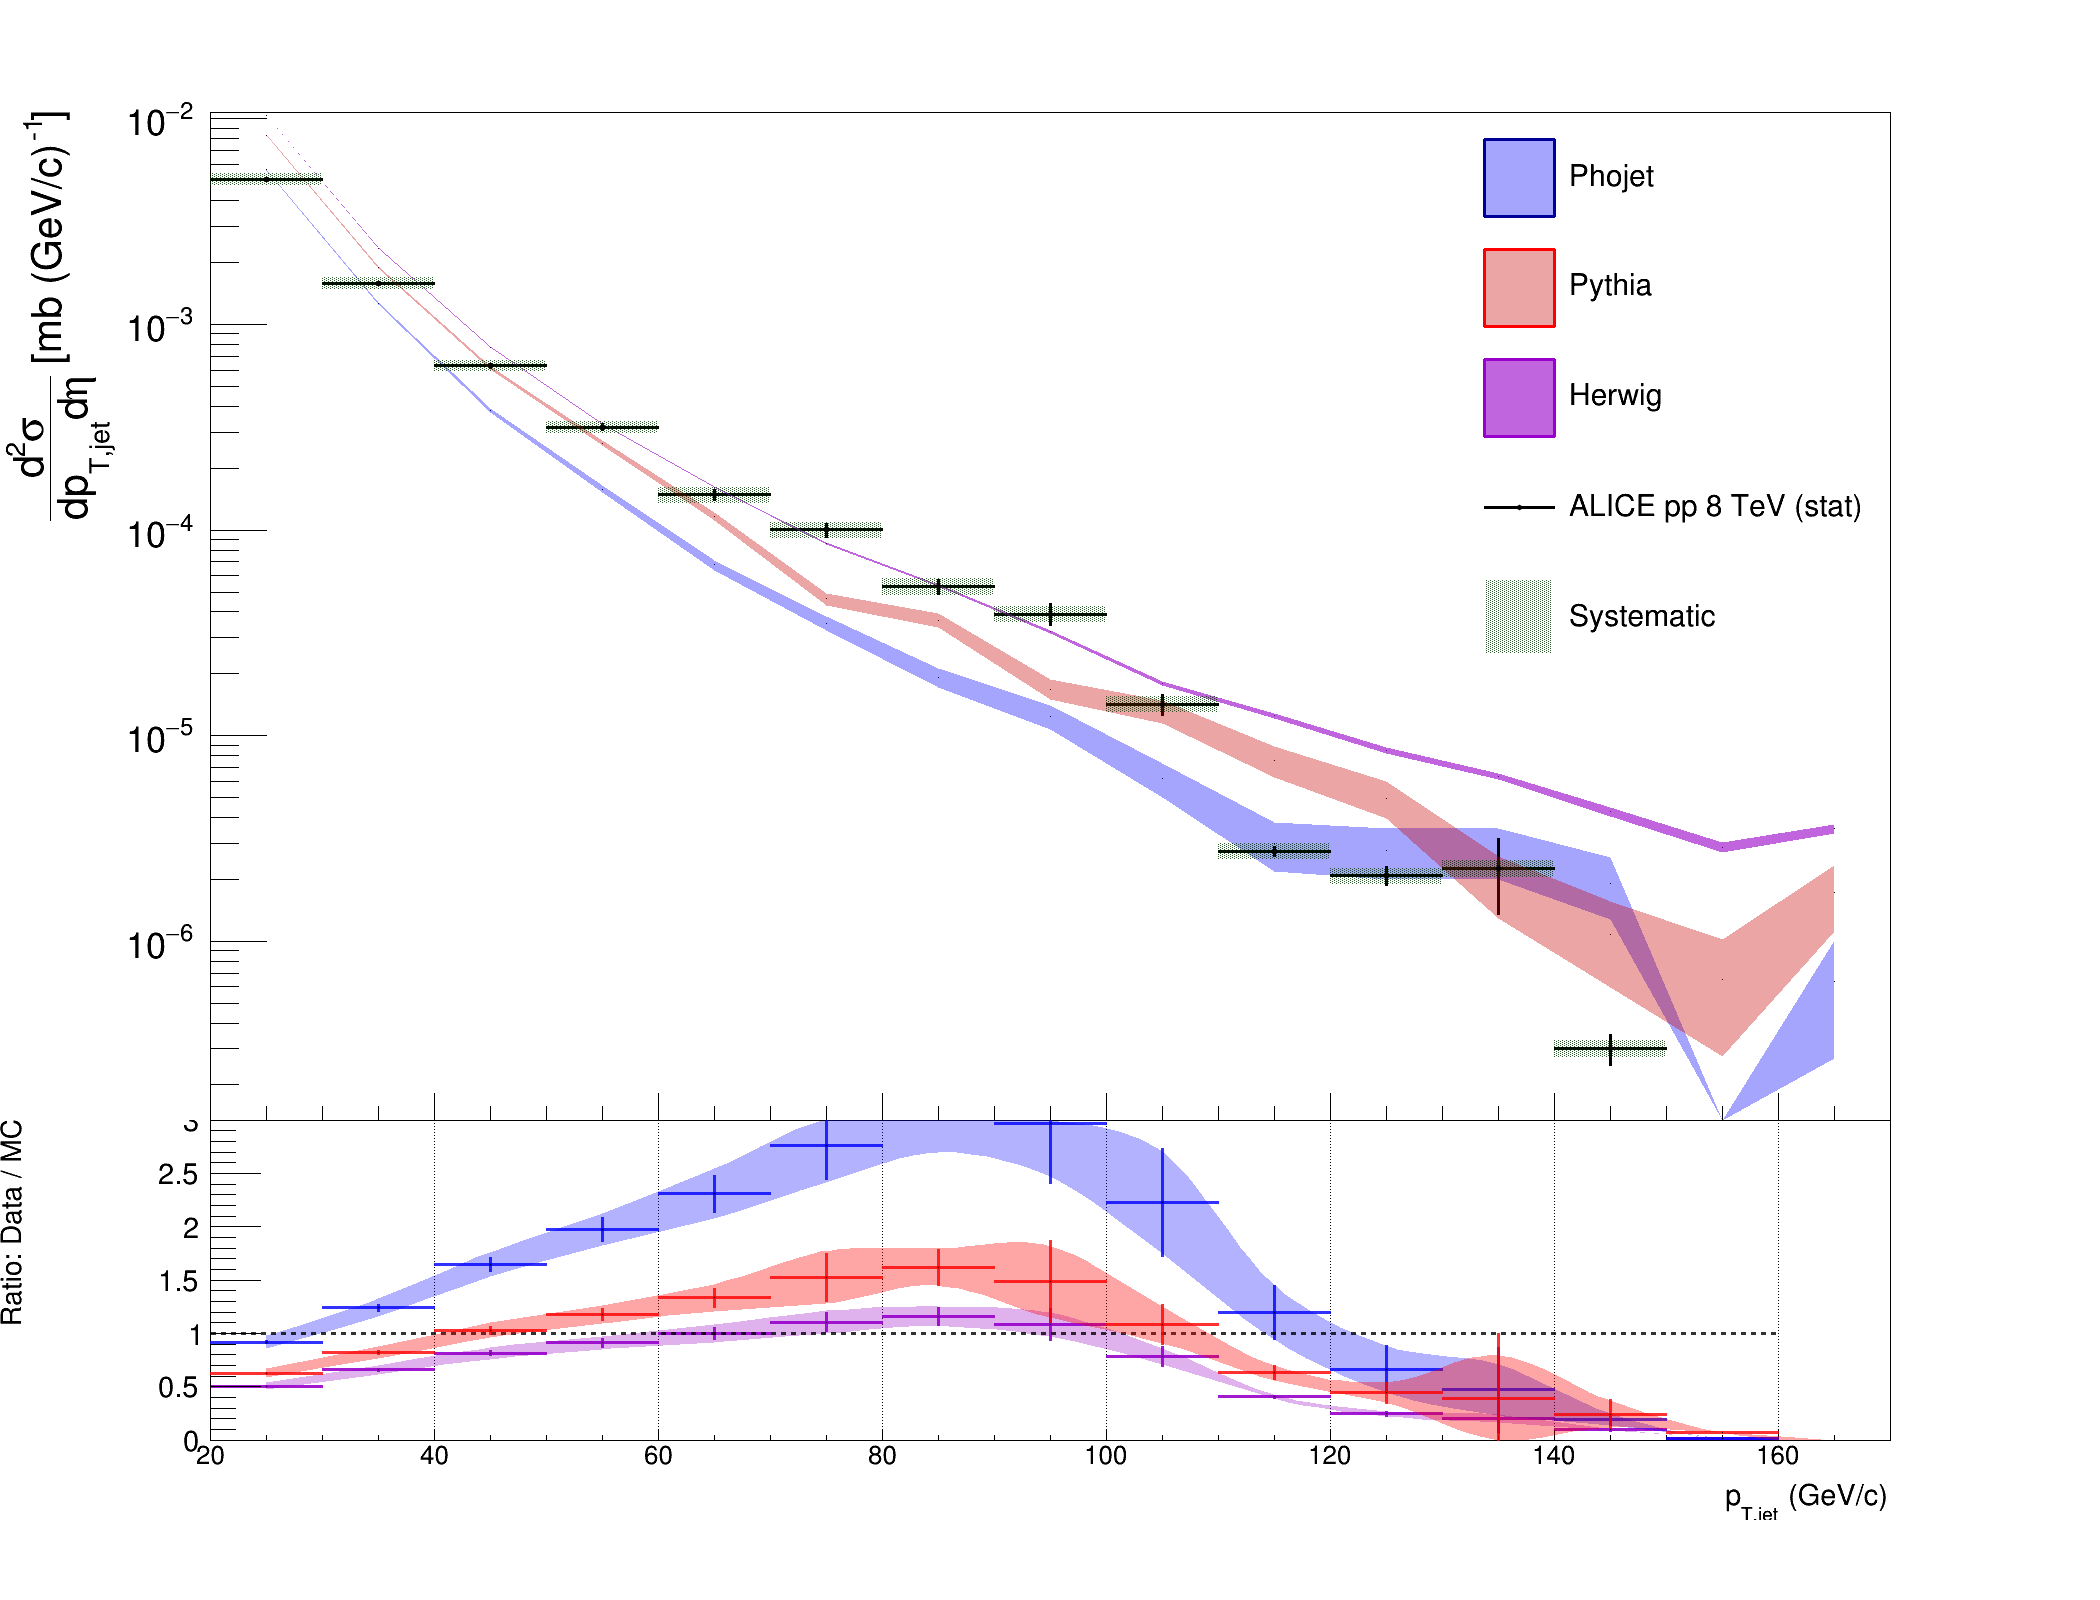
\includegraphics[width=8.5cm]{XSecR03}
\centering
\caption{8 TeV inclusive jet differential cross-section for R = 0.3.}
\label{fig:JetXsecR03}
\end{figure}

\begin{figure}[h]
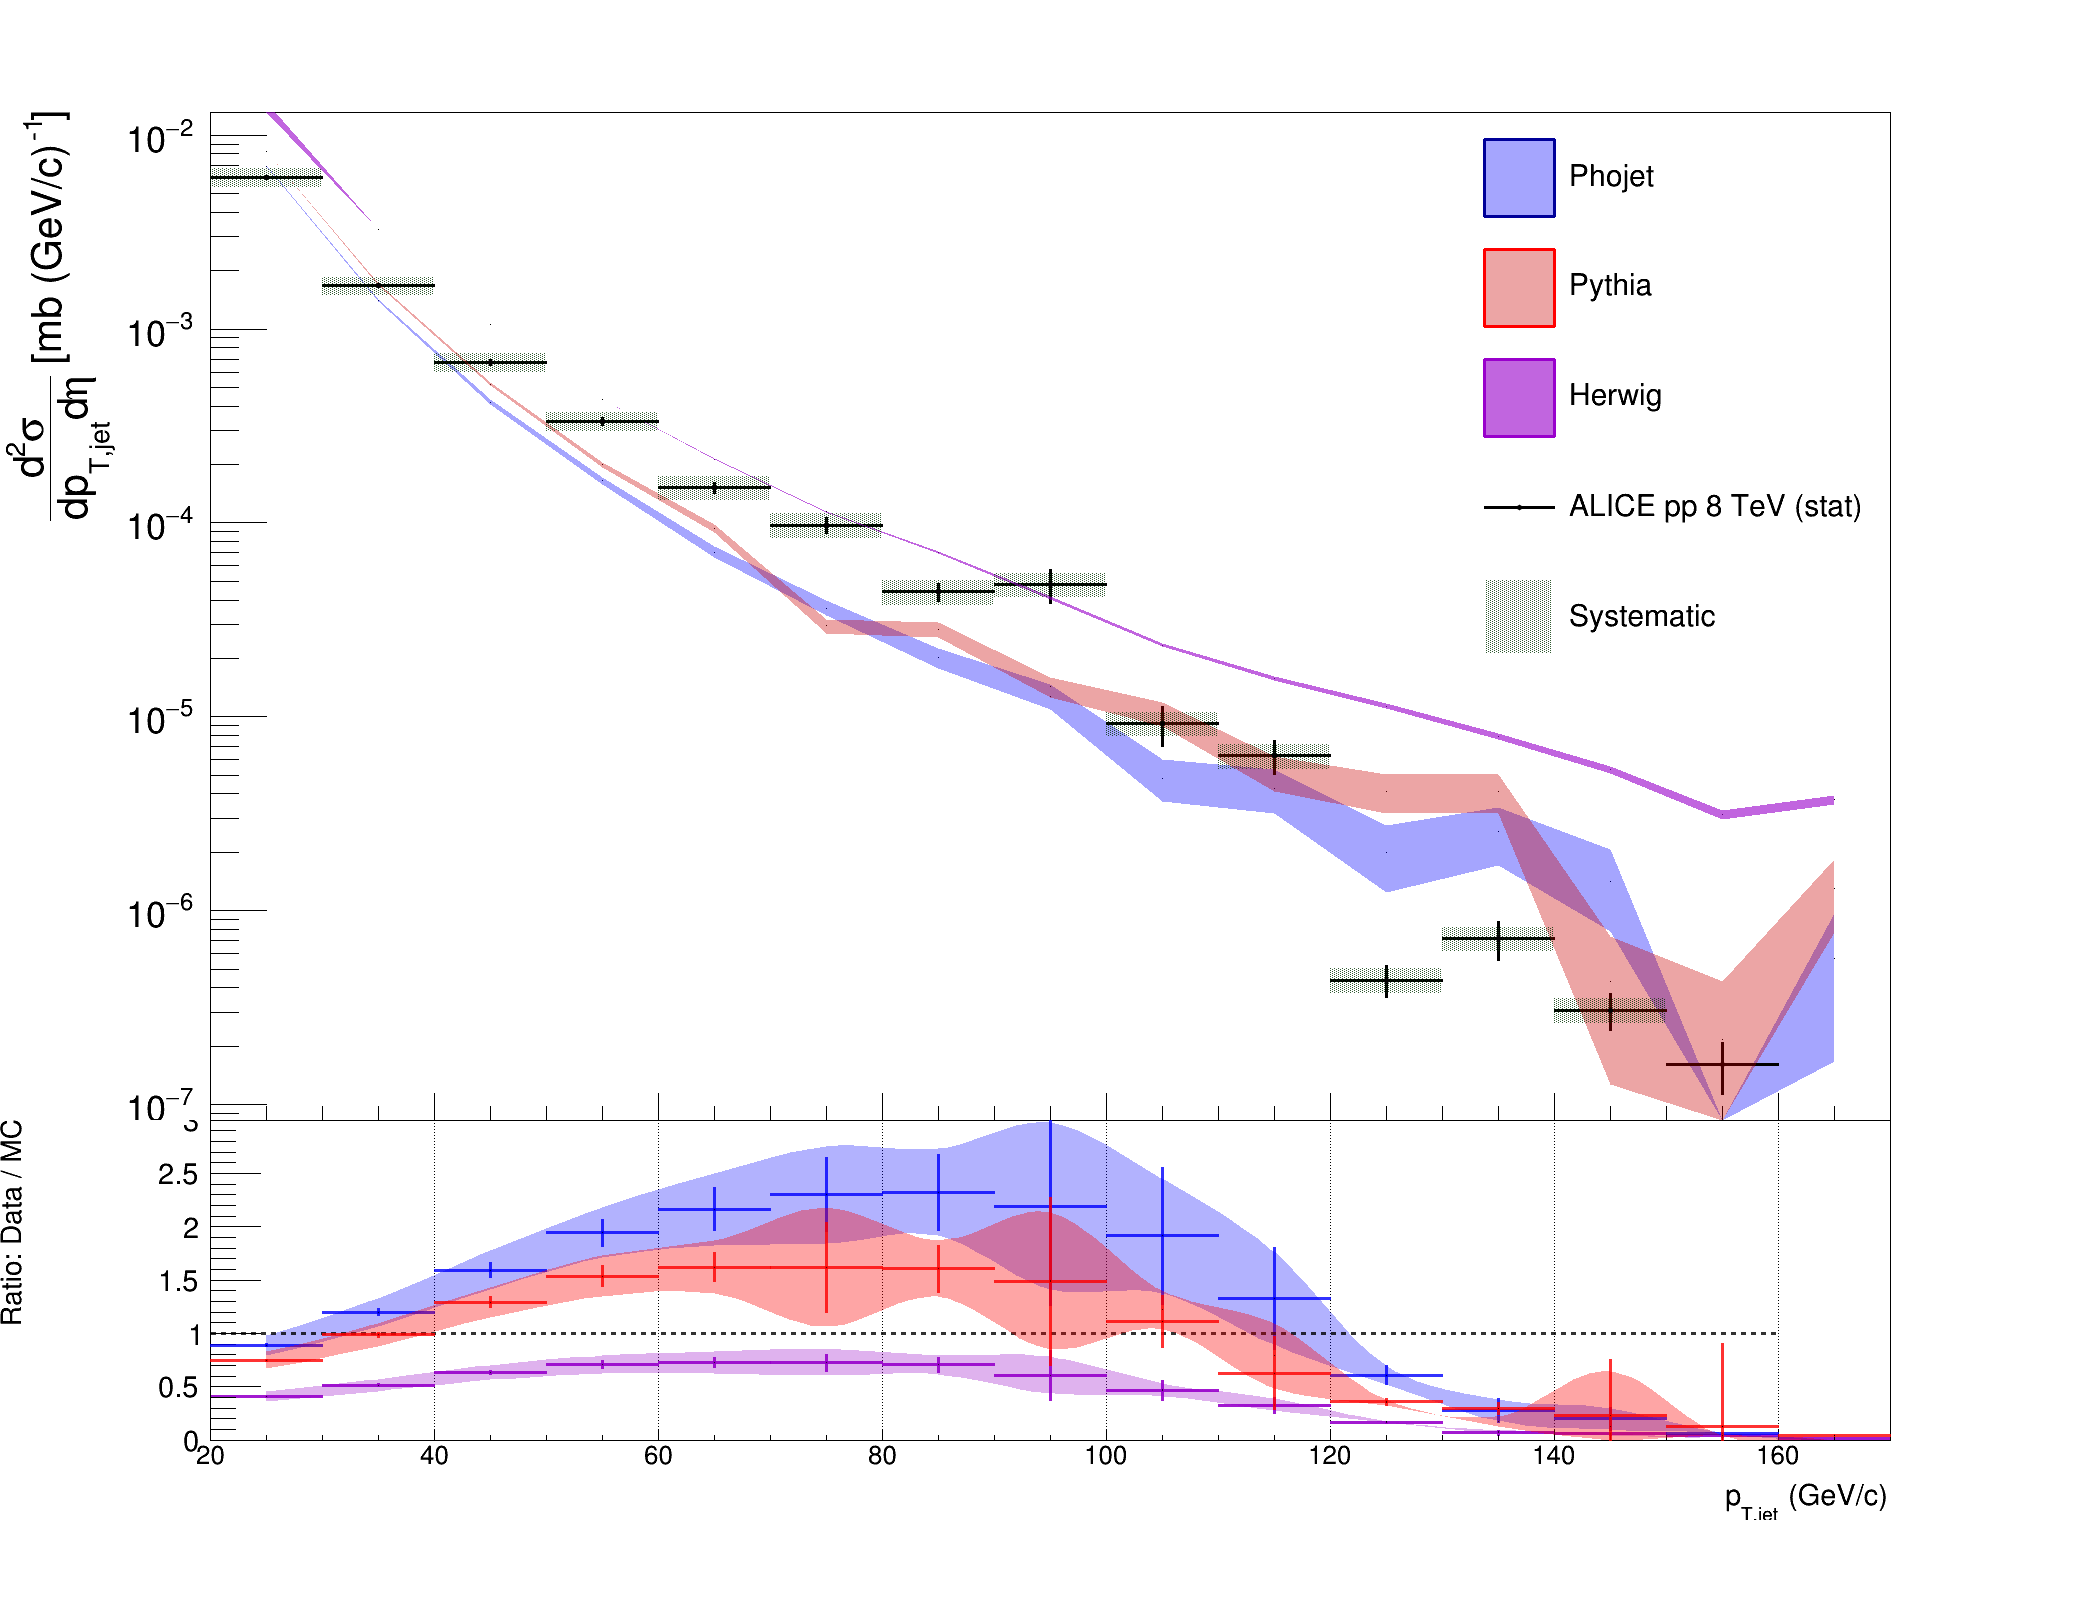
\includegraphics[width=8.5cm]{XSecR04}
\centering
\caption{8 TeV inclusive jet differential cross-section for R = 0.4.}
\label{fig:JetXsecR04}
\end{figure}

Figures \ref{fig:JetXsecR02}, \ref{fig:JetXsecR03}, and \ref{fig:JetXsecR04} show the inclusive jet cross-sections from R = 0.2 through R = 0.4.  The figures are split into two sections.  The cross-sections as measured from ALICE along with the associated statistical errors are shown in black.  The associated systematic errors from the ALICE measurements are shown as the green shaded area.  Min Bias Monte Carlo generated events from Pythia (Red), PHOjet (blue), and Herwig (magenta) are showen as colored bands to convey the statistical uncertainties from each simulation.  On the bottom half of each plot are the relative ratios of the ALICE jet cross-sections to one of the Monte Carlos using the same color scheme as above.  

What can we tell from these results?  First, we can see that the cross-sections are measured over a wide range, about five orders of magnitude, between 20 GeV/c to 160 GeV/c in $p_{T}$.  The R = 0.2 and R = 0.3 cross-sections show a well defined trend between 20 GeV/c - $\sim$100 GeV/c, after this point the data hard jerk after which the data points show wider fluctuations.  This same trend is seen in the R = 0.4 jet cross-section but the jerk happens earlier in $p_{T}$ around  80 GeV/c.  The fluctuations are most likely an artifact of the bin-by-bin corrections and the lack of EMCal trigger simulations as discussed in Chapter \ref{ch:analysis}.  

Comparing the data to the Monte Carlos we see that the two simulations, Pythia and PHOjet, produced by the ALICE Collaboration tend to under predict the data.  PHOjet has the least agreement with the data.  The poor agreement with PHOjet can be explained by the fact that PHOjet is an older Monte Carlo generator and better tuned to describing lower energy experiments from the past.  The Monte Carlo Simulation from Herwig was produced on a local server farm at the University of Tennessee and we see that reflected in the low statistical errors.  The Herwig data tends to over predict the data.  Both Herwig and Pythia agree well with the data between 20 GeV/c to 100 GeV/c.  It is hard to say that one is `better' then the other because of the relatively large statistical errors from Pythia.  However, for the R = 0.4 jet cross-section we can see thatthe data seems to trend better towards the clusterization theory of hadroization used in Herwig.

Through scaling these results may also serve as a reference for heavy-ion collisions and help to better constrain our understanding of parton energy loss mechanisms in the QGP.  


\subsubsection{Jet Cross-Section Ratios}

\begin{figure}[h]
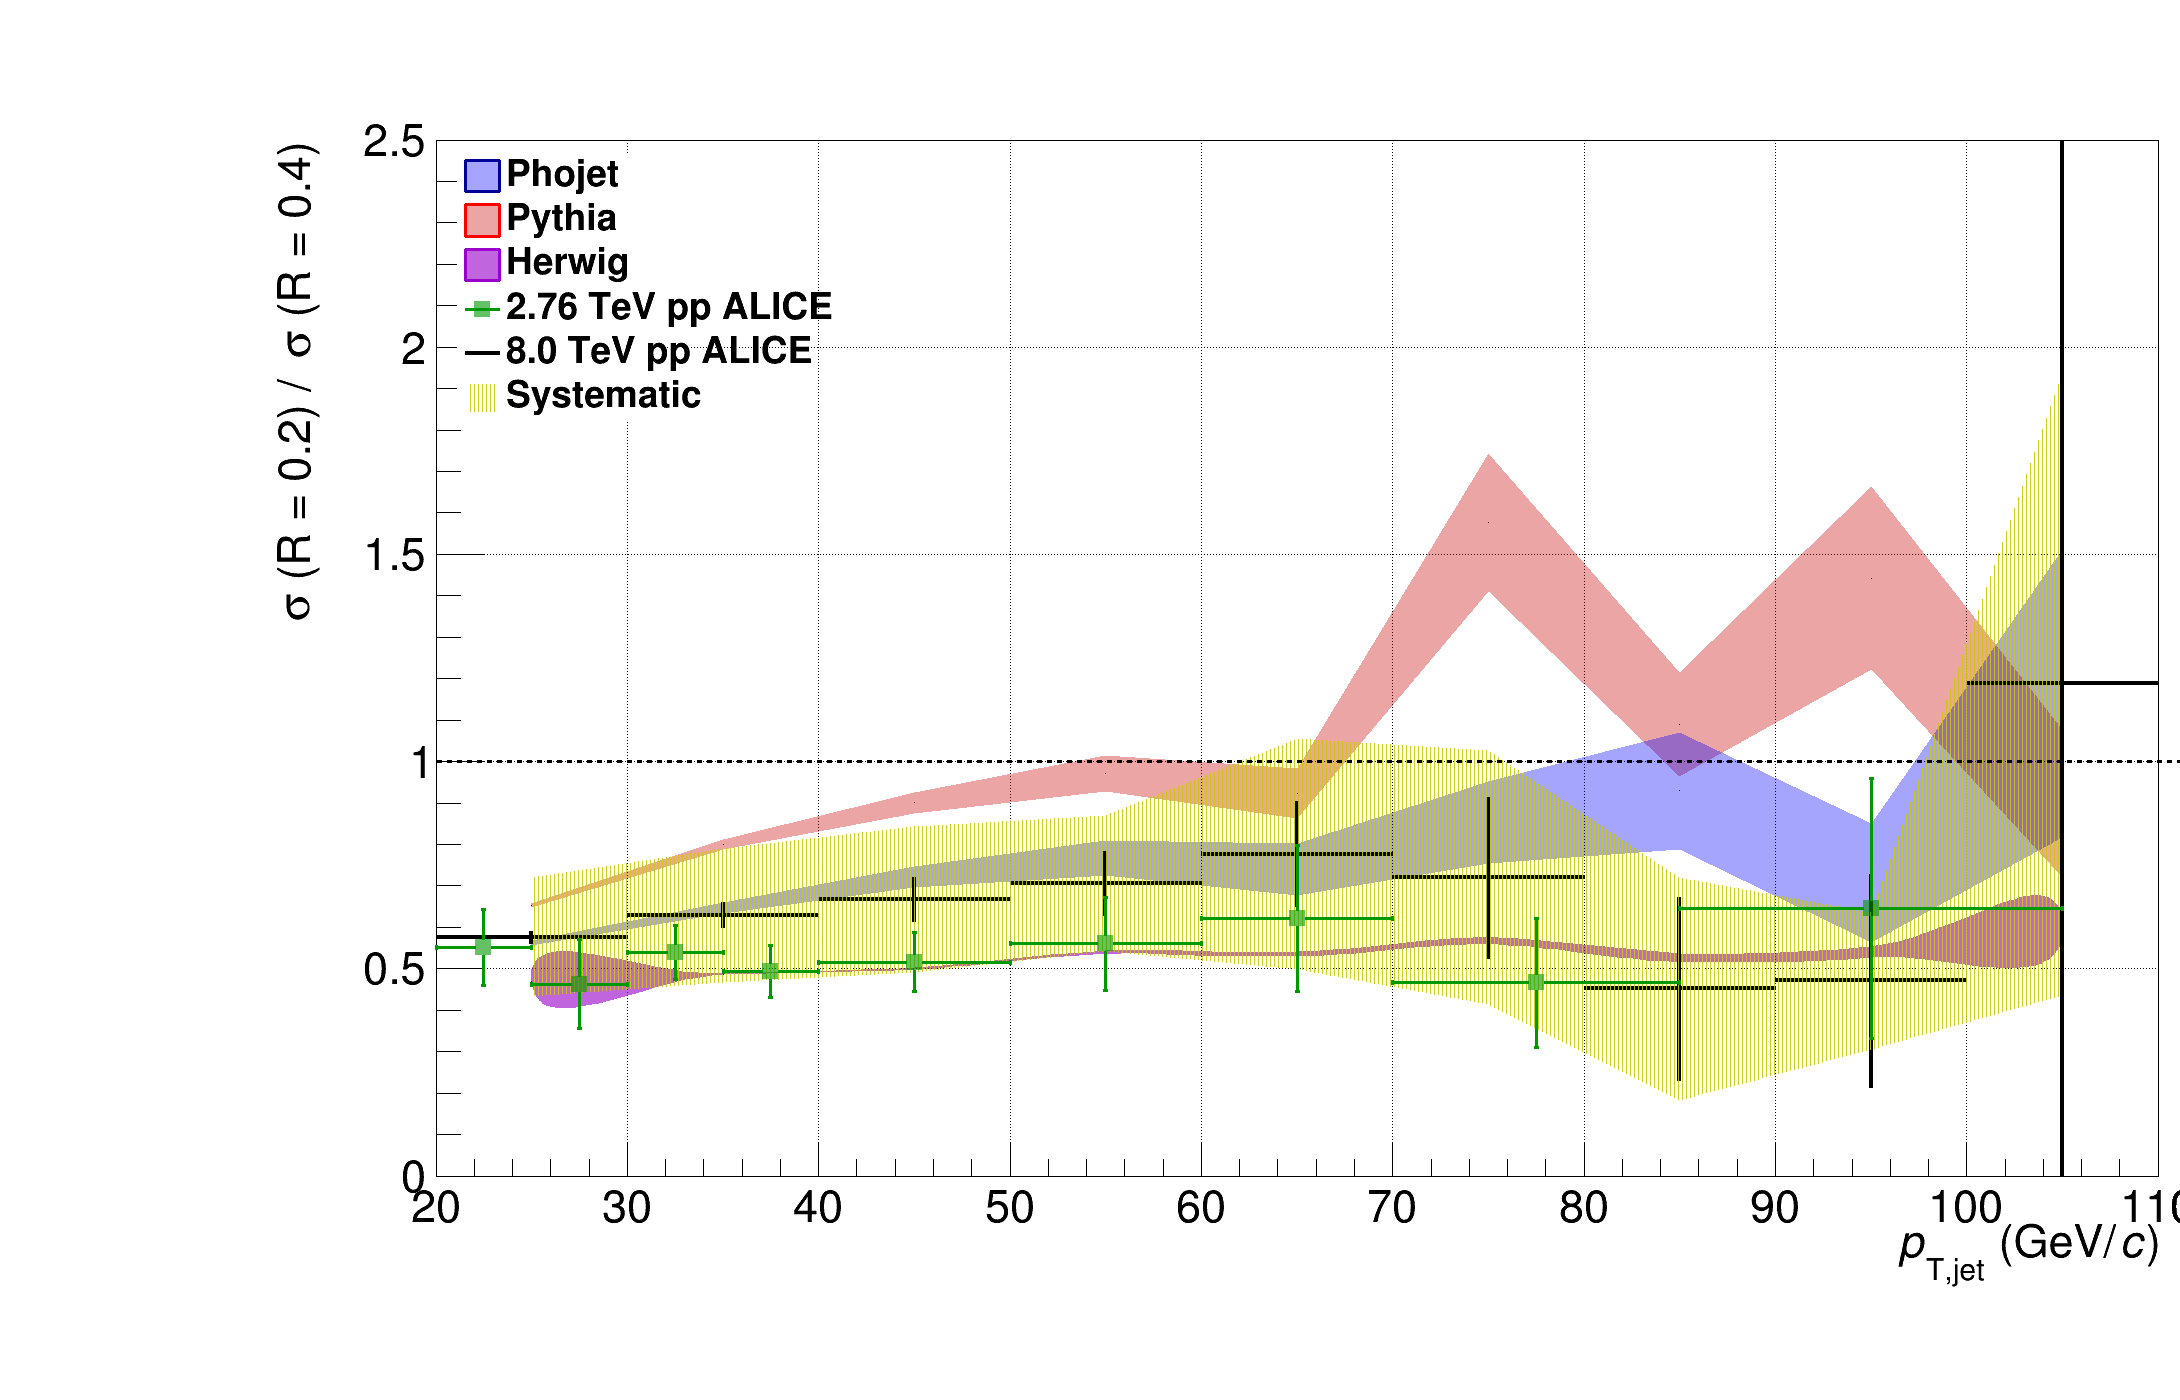
\includegraphics[width=8.5cm]{XSecRatioR02}
\centering
\caption{Ration of the jet cross-sections R = 0.2  to R = 0.4.}
\label{fig:JetXsecRatioR02}
\end{figure}

\begin{figure}[h]
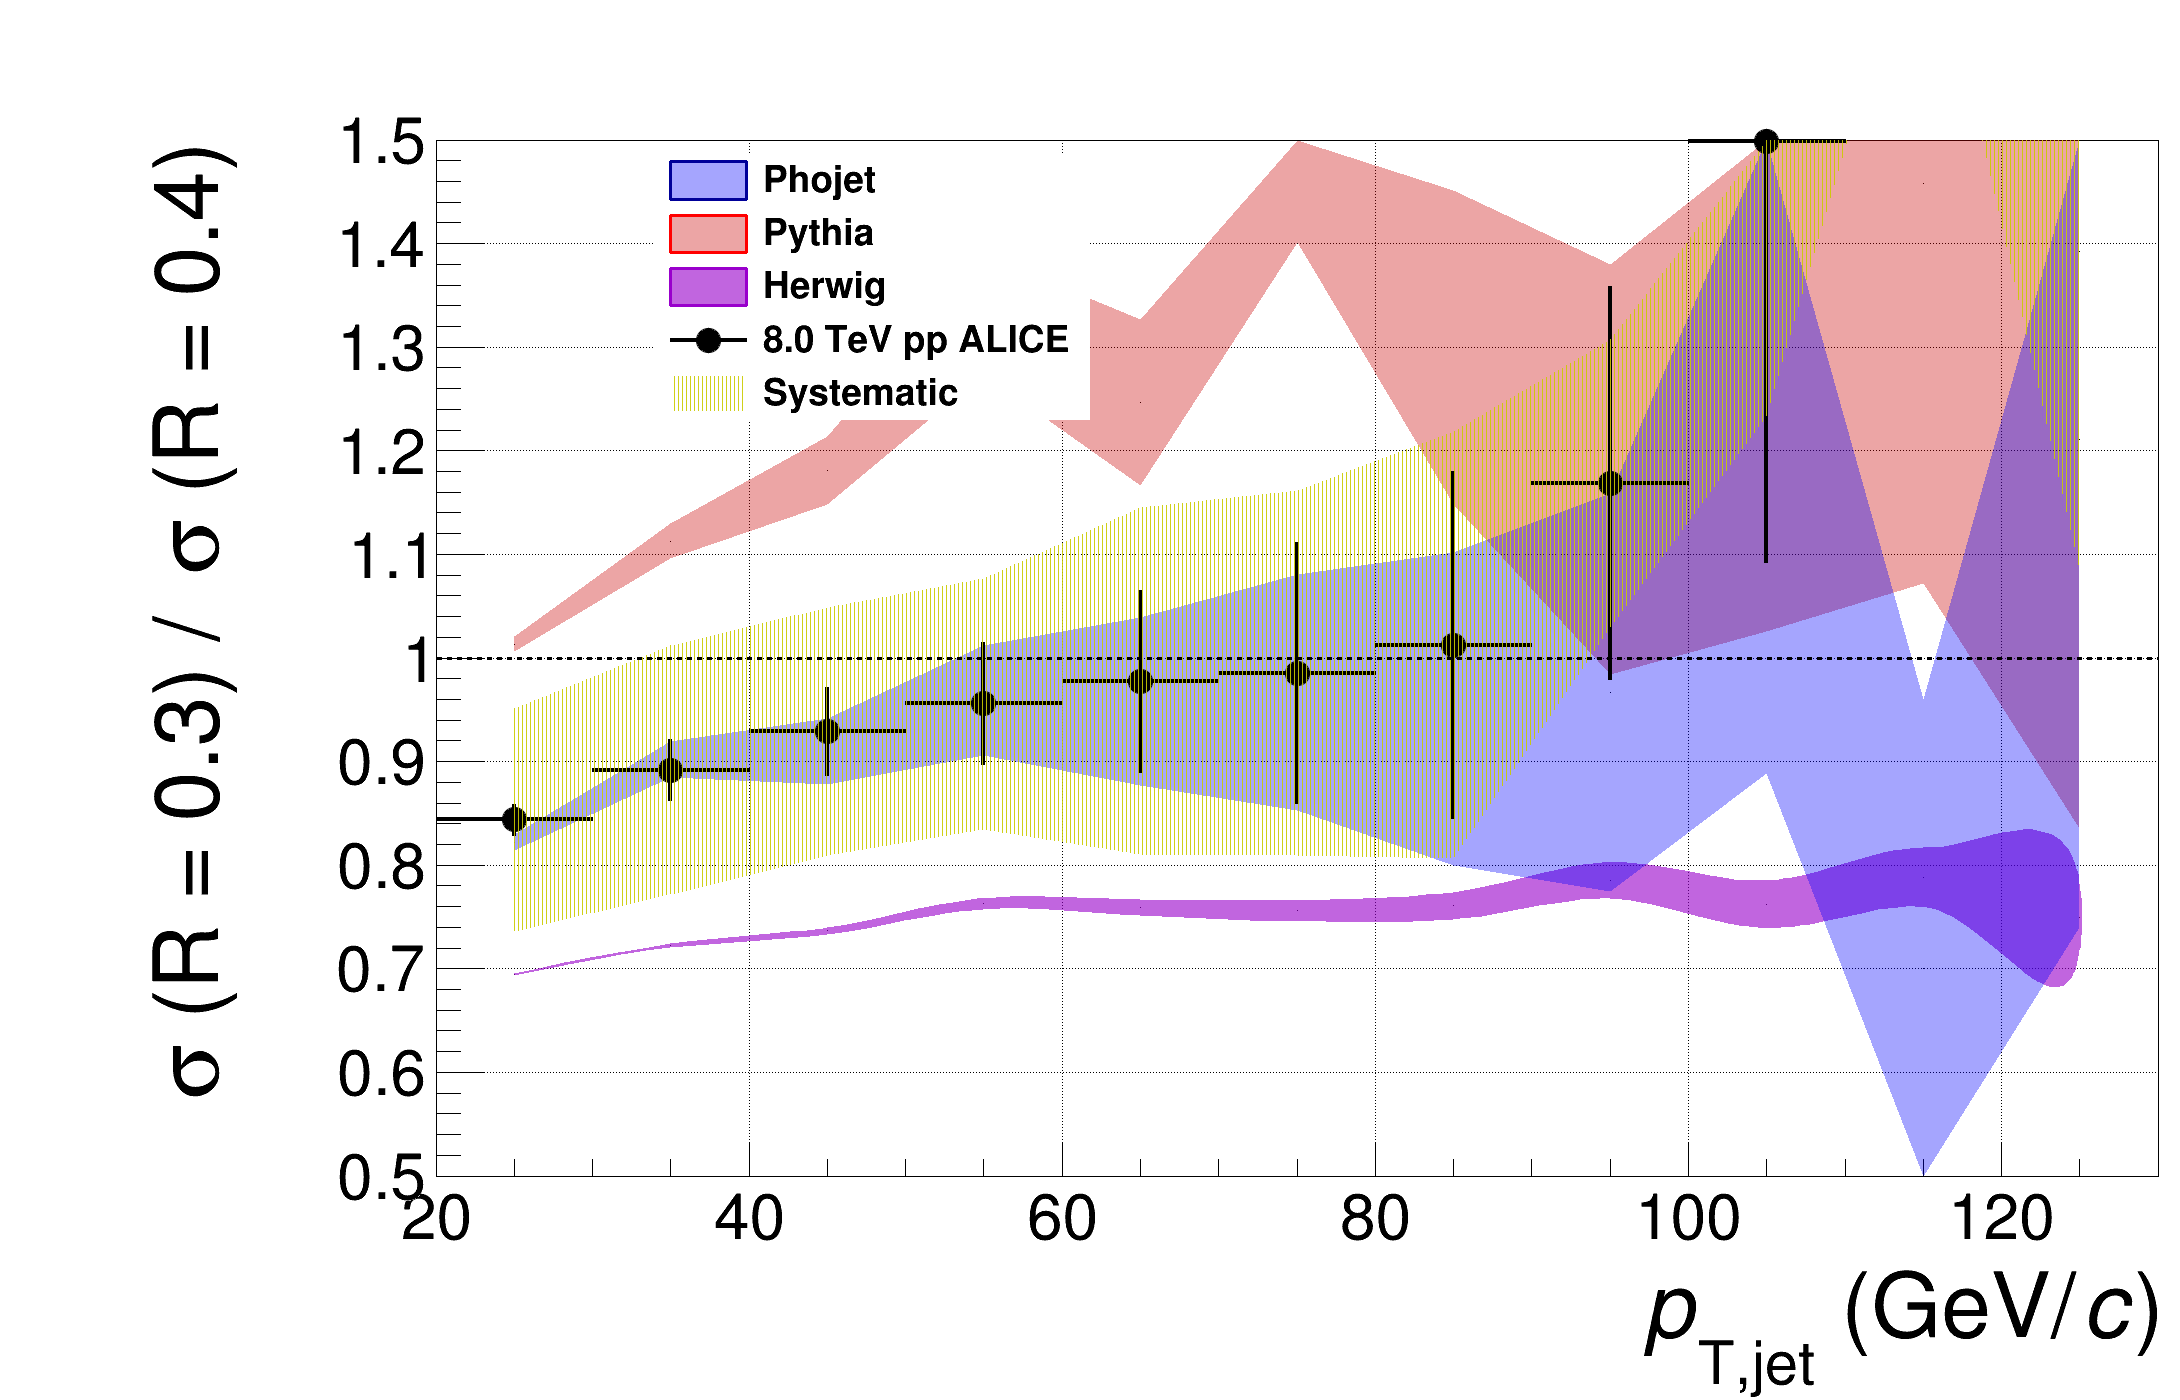
\includegraphics[width=8.5cm]{XSecRatioR03}
\centering
\caption{Ration of the jet cross-sections R = 0.3  to R = 0.4.}
\label{fig:JetXsecRatioR03}
\end{figure}


\begin{figure}[h]
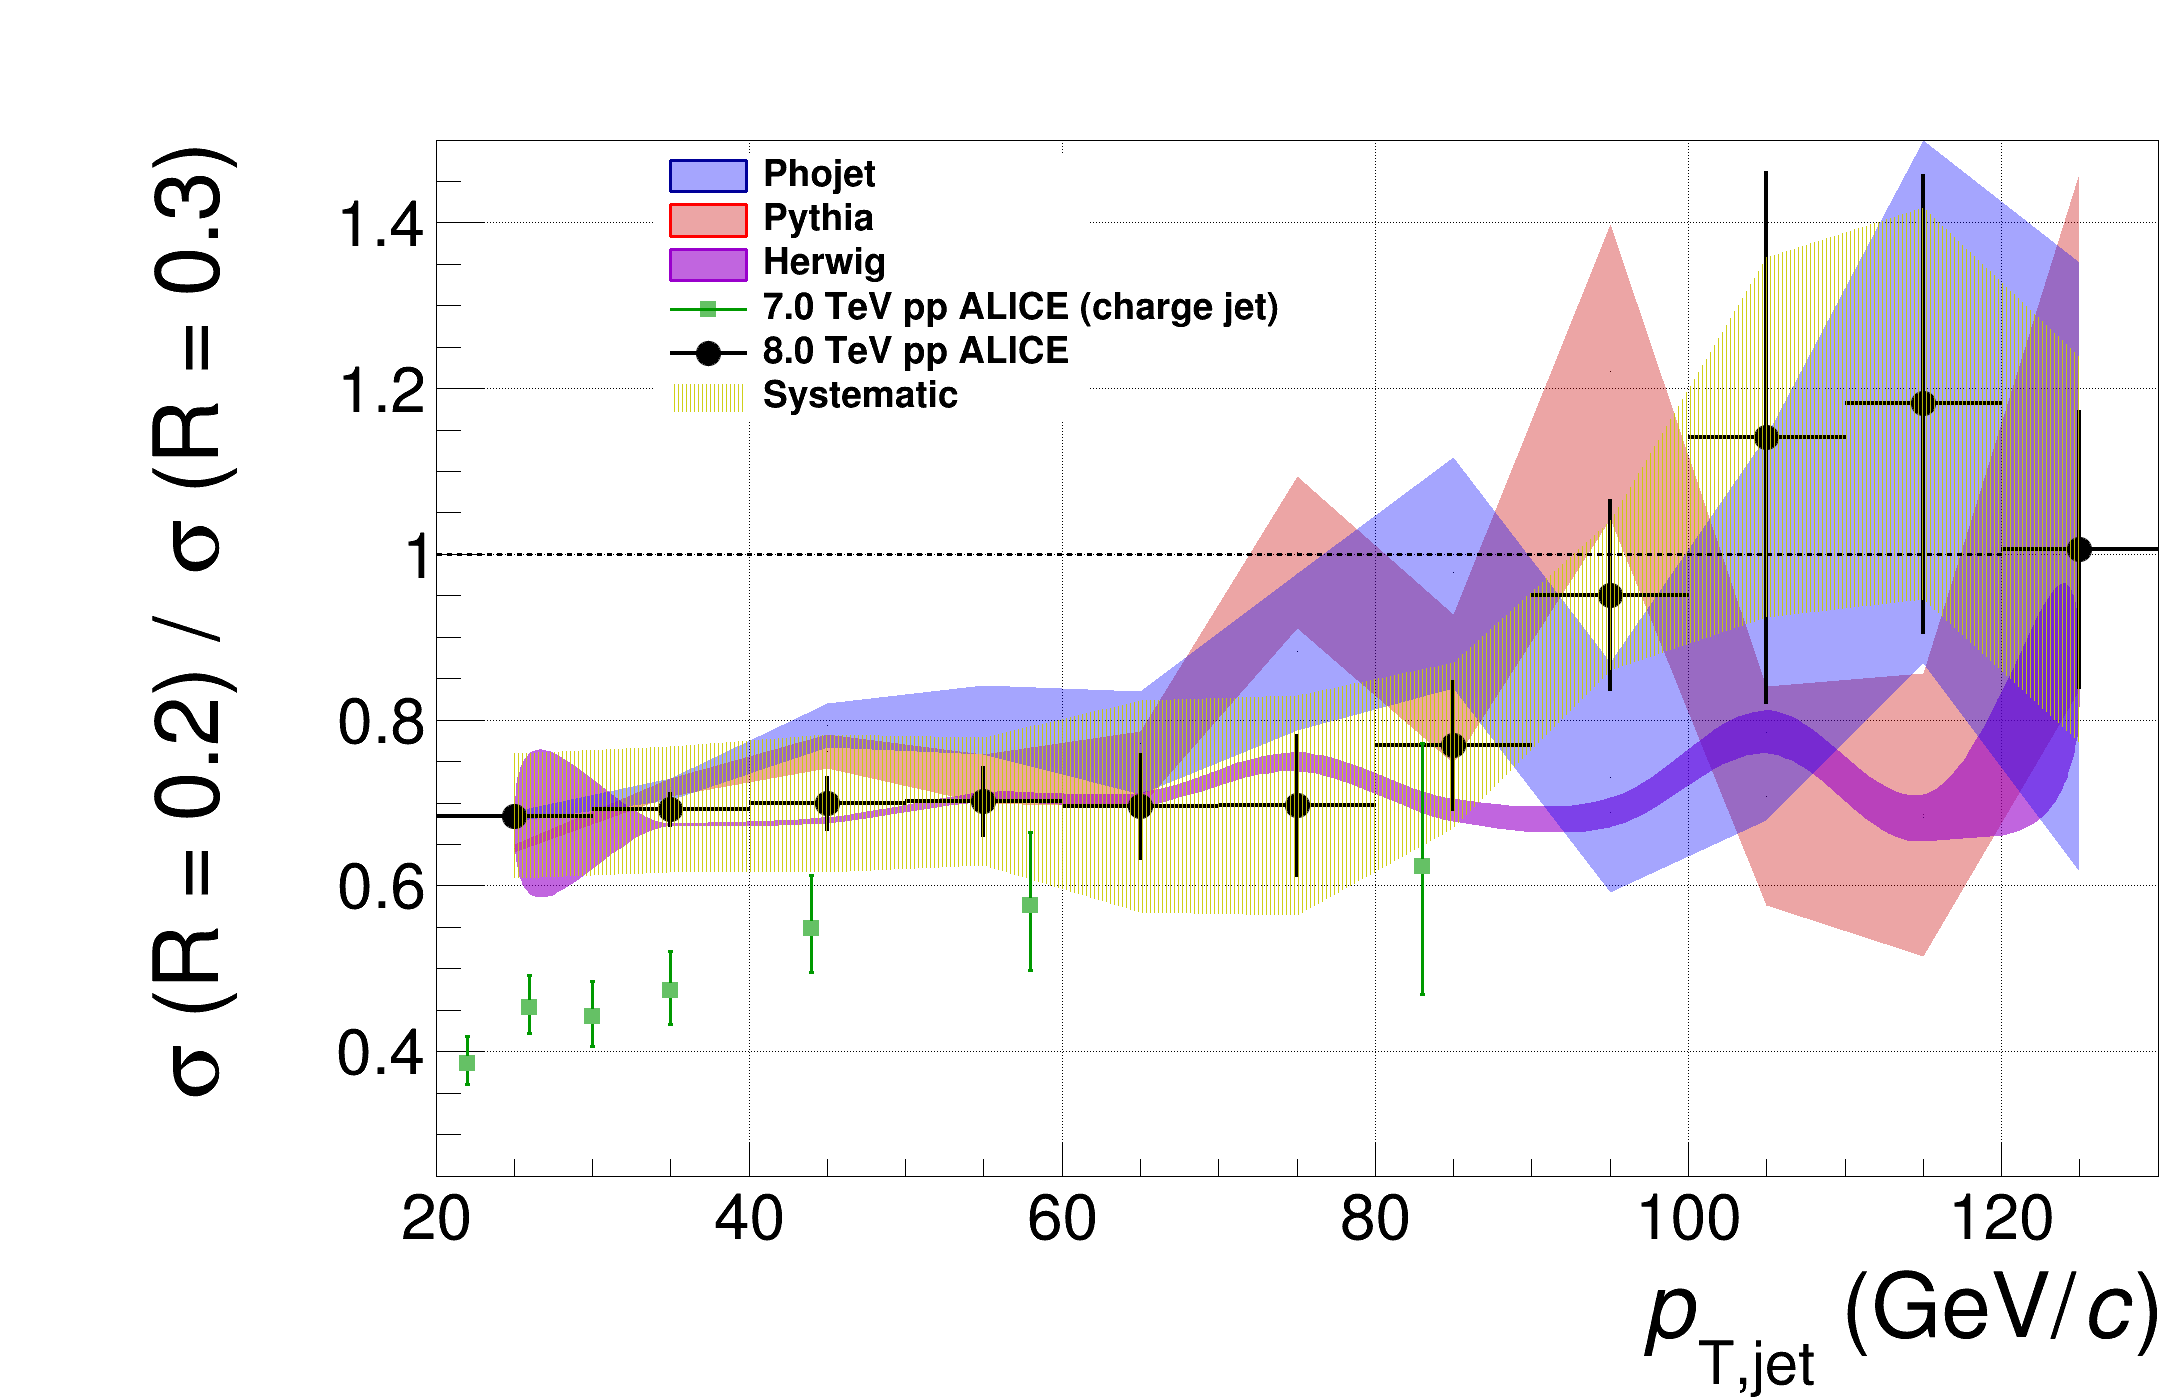
\includegraphics[width=8.5cm]{XSecRatioR023}
\centering
\caption{Ration of the jet cross-sections R = 0.2  to R = 0.3.}
\label{fig:JetXsecRatioR023}
\end{figure}


\newpage

The ratio of the jet cross sections as a function of the jet radii is defined as,

\begin{equation}
\mathscr{R} (p_{T}; \, R_{1},R_{2}) = \frac{d\sigma(R_{1} /d\eta \, dp_{T}) }{d\sigma (R_{2} /d\eta \, dp_{T})},
\label{eq:jetxsecratio}
\end{equation}

\noindent
where $R_{1}$ and $R_{2}$ are the jet radii in question. This probes the transverse structure of jets and is sensitive to QCD hardonization\cite{SOYEZ201159}.  Figures \ref{fig:JetXsecRatioR02}, \ref{fig:JetXsecRatioR03}, and \ref{fig:JetXsecRatioR023} report the ratios of the jet cross-sections between R = 0.2 / R = 0.4, R = 0.3 / R= 0.4, and R = 0.2 / R = 0.3 respectively.  The figures also show the relative ratios plotted from the 8 TeV ALICE data, Pythia, PHOjet, and Herwig using the same color schema as from the jet cross-sections.  Errors between the cross-sections of different radii are considered uncorrelated and added in quadrature to form the error bars reported in the figures.

A similar analysis to this thesis was performed using a 2.76 TeV  data sample collected from ALICE\cite{MA2013319} and it is compared to Figure \ref{fig:JetXsecRatioR02} and \ref{fig:JetXsecRatioR023} in green bullet points.  In order to avoided double counting by sampling the same jet  found using an R = 0.2 and R = 0.4 jet finding algorithm these ratios use disjointed samples of the 8 TeV data set.  From the results of the cross-section ratios we see that the 8 TeV data as reported from this thesis agrees well 2.76 TeV results from ALICE in Figure \ref{fig:JetXsecRatioR02}.  Interestingly it seems that for all three of the figures the PHOjet Monte Carlo agrees well with the data and is the only simulation that agrees for the $\sigma (R = 0.3)$ / $\sigma (R = 0.4)$ ratio.  It can be concluded that the Pythia ratios have the least agreement because it only includes the LO matrix to calculate partonic showers which does not model the angular ordering of QCD radiation very well.  Herwig tends to under predict the data, especially at low-$p_{T}$, which is expected and may be understood in terms of limitations modeling low energy background particles with tune used in this thesis (v2.3).  Similar to the previous results these ratios can be used to constrain jet quenching in the QGP.  These results also report the first ratio of jet-cross sections between R = 0.2 and R = 0.3.  These is especially helpful for heavy-ion collisions as most jet results from heavy-ions use either an R = 0.2 or R = 0.3 jet radius as this helps suppress the background in the high multiplicity environment.











\iffalse

CMS\cite{CMS:2013kda} and ATLAS\cite{Aaboud:2017dvo} both reported the double differential cross section for inclusive jets at 8 TeV.  

\begin{figure}[h]
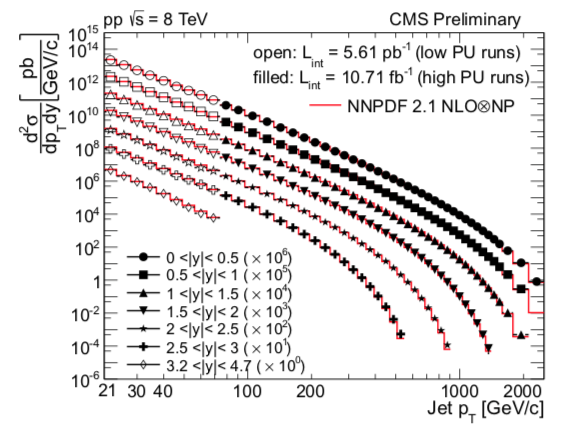
\includegraphics[width=10.0cm]{CMS8TeVJet}
\centering
\caption{8 TeV CMS inclusive jet cross sections with radii of R = 0.7 and binned by jet rapidity compared to NLO calculations with non-pertubative corrections\cite{CMS:2013kda}.}
\label{fig:CMS8TeVRescale}
\end{figure}

\begin{figure}[h]
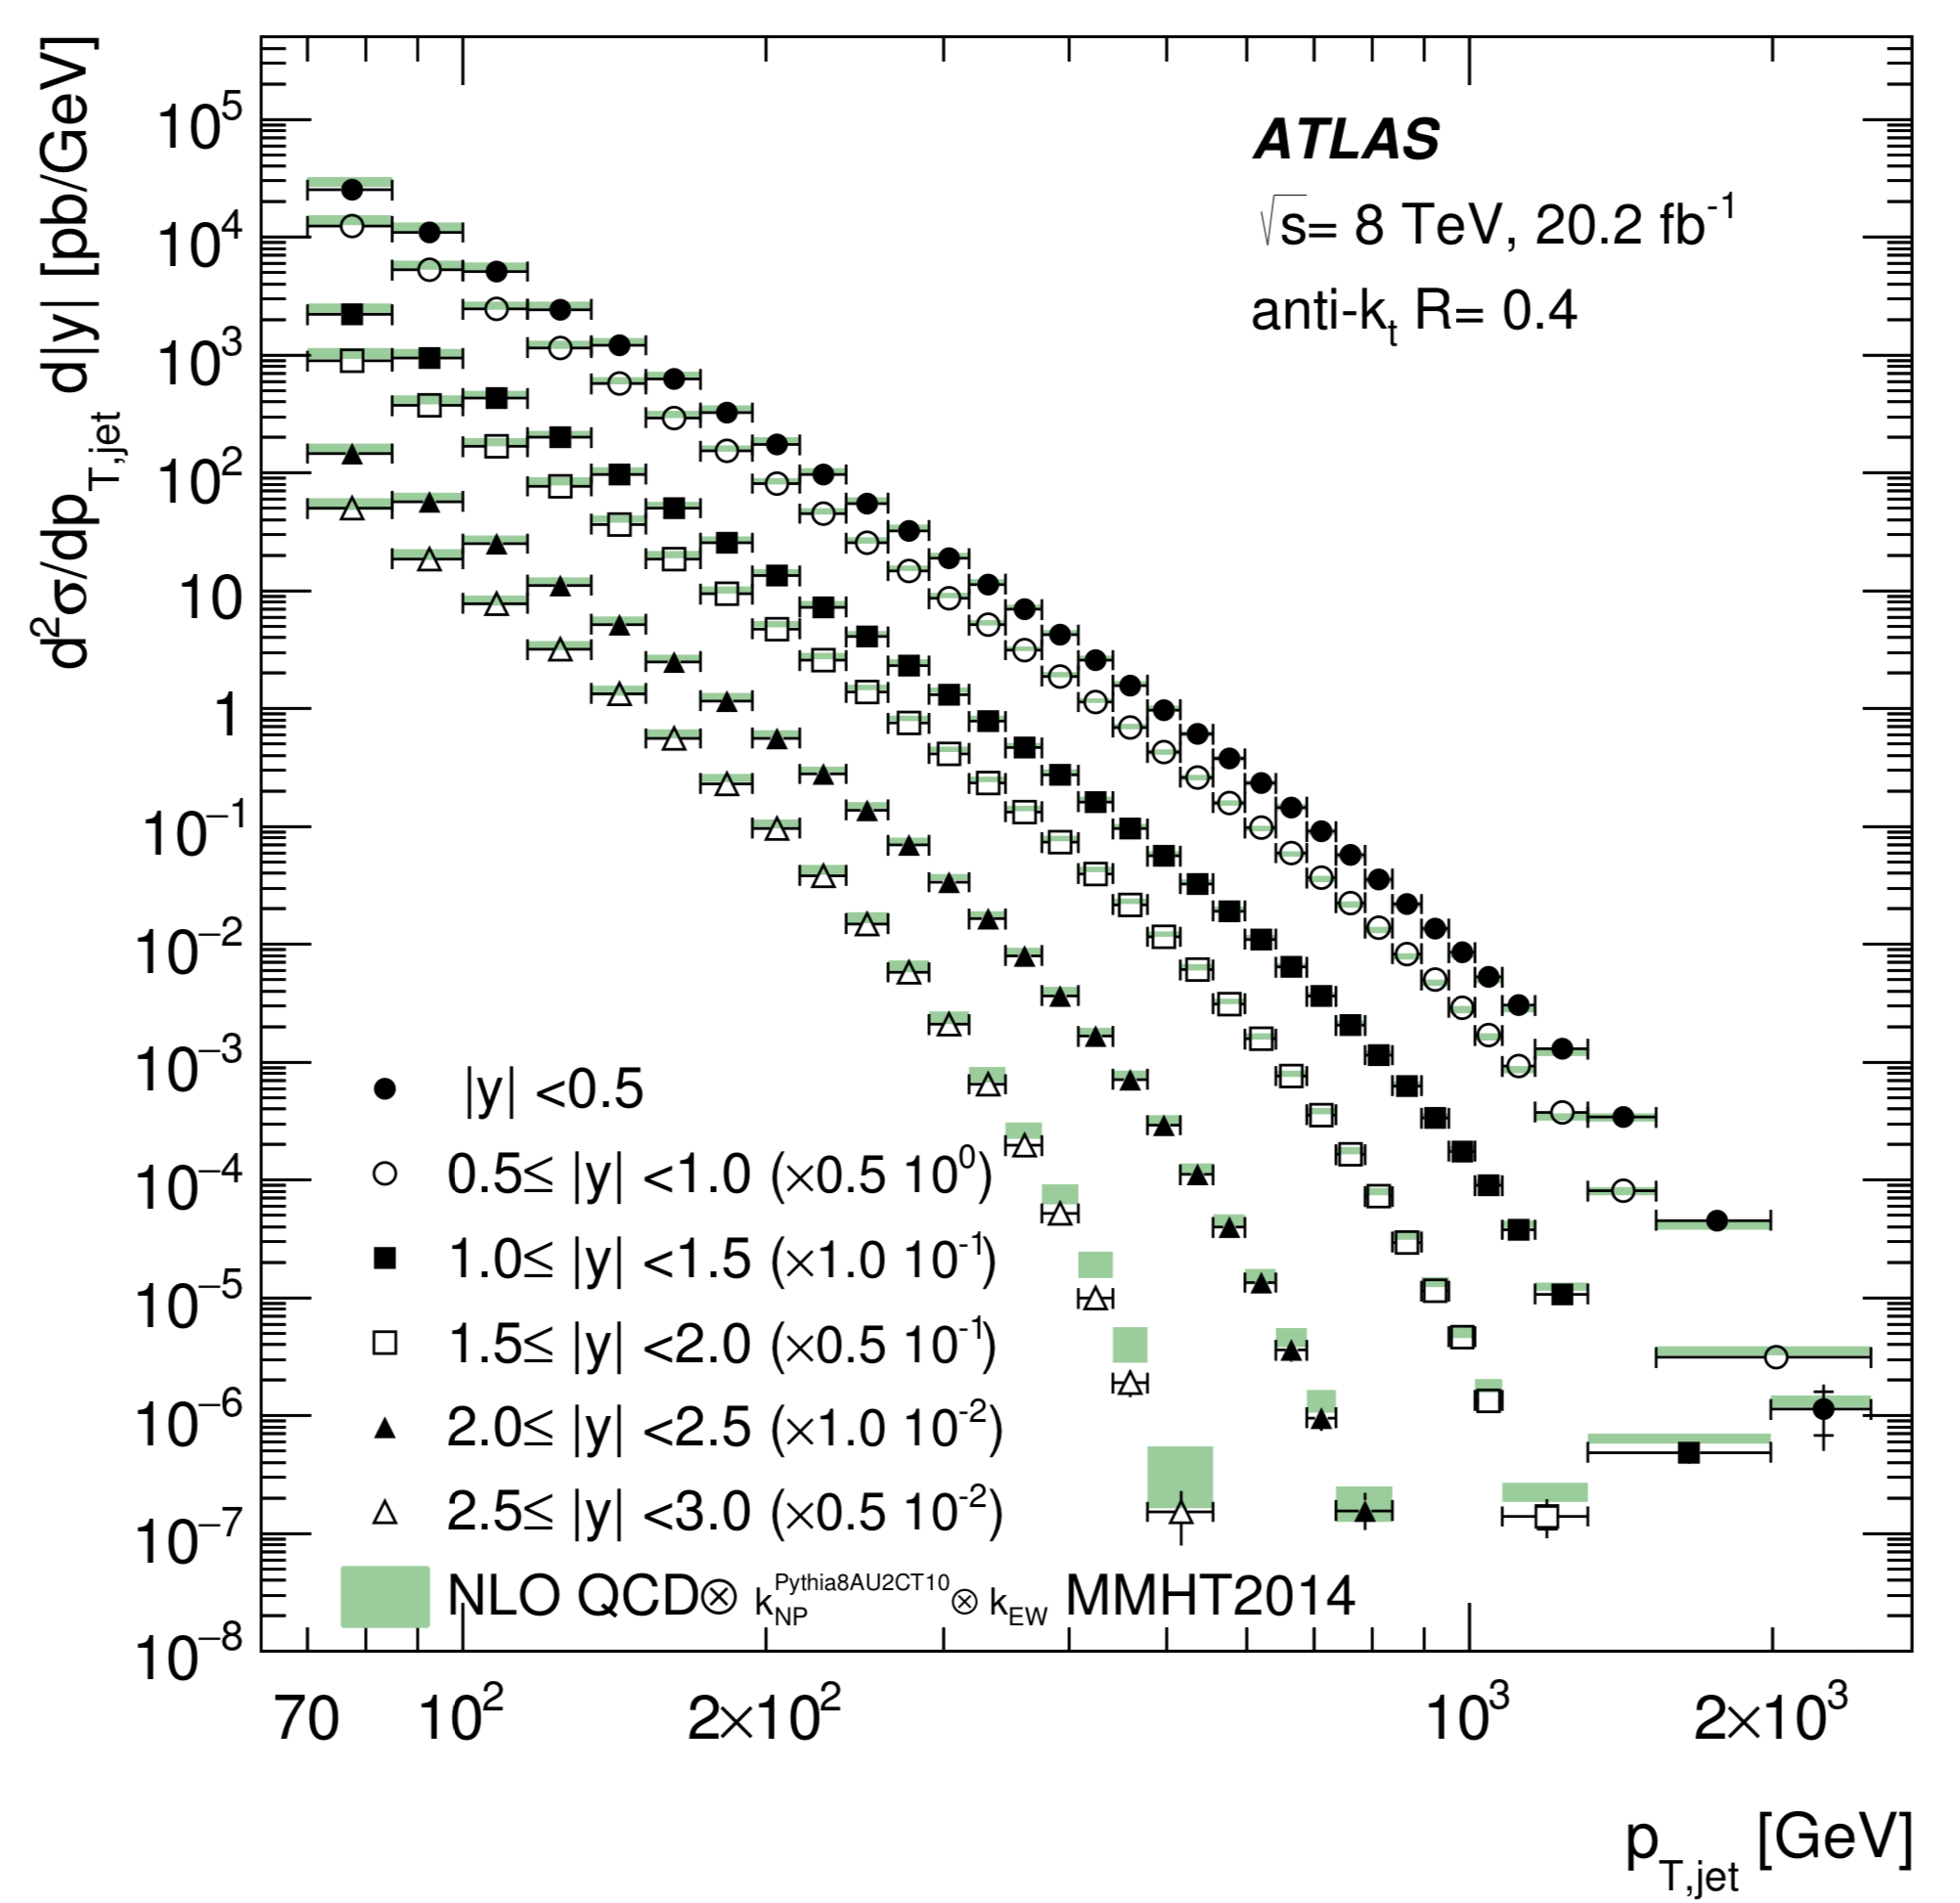
\includegraphics[width=10.0cm]{ATLAS8TeVJet}
\centering
\caption{R = 0.4 inclusive jet cross section at 8 TeV from ATLAS in binned by jet rapidity compared to NLO QCD predictions\cite{Aaboud:2017dvo}.}
\label{fig:ATLAS8TeV}
\end{figure}

\begin{figure}[h]
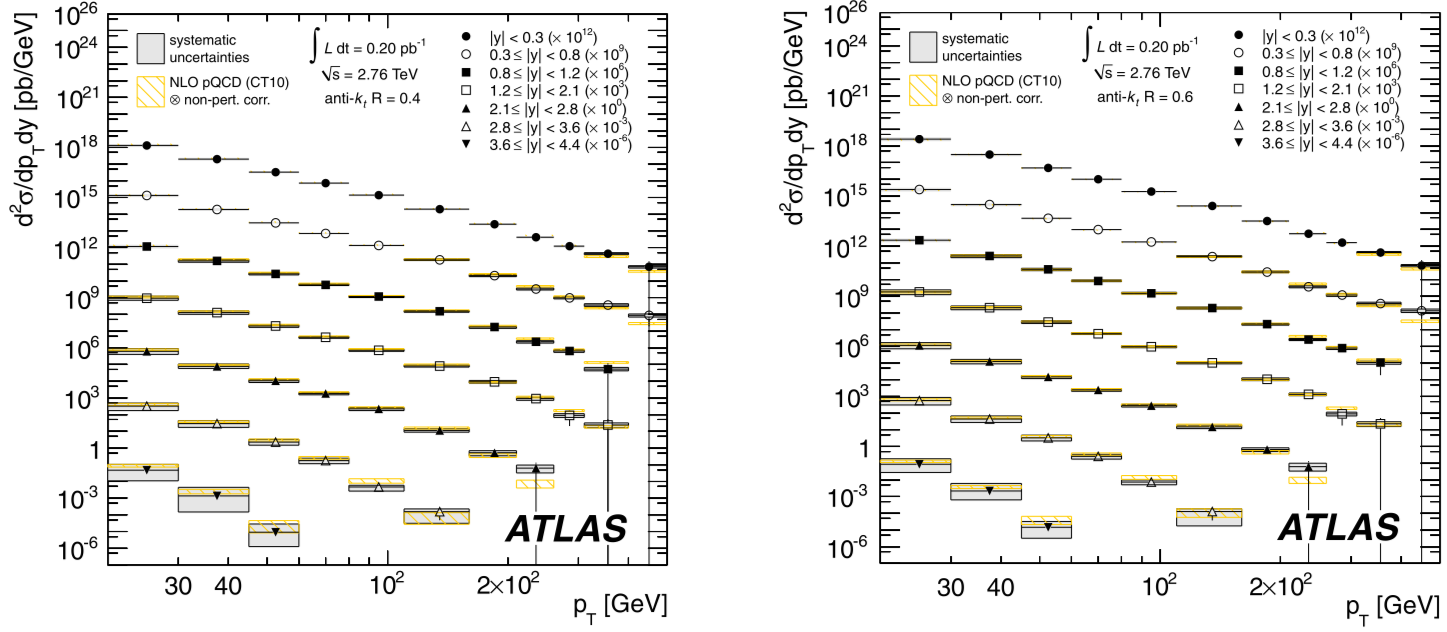
\includegraphics[width=14.0cm]{ATLAS8TeVJetRecaled}
\centering
\caption{The 8 TeV ATLAS jet cross sections rescaled to better show comparissons with NLO and non-pertubative calculations at low $p_{T}$\cite{Aaboud:2017dvo}.}
\label{fig:ATLAS8TeVRescale}
\end{figure}

\section{Inclusive Jet Spectra and Cross Section Ratios at 2.76 TeV}
Inclusive jet spectra and cross section ratios were measured in the ALICE experiment using a 2011 pp 2.76 TeV data sample\cite{MA2013319}.  Jets were reconstructed using TPC tracks and EMCal clusters with the FastJet Anti-$K_{T}$ algorithm.  Tracks with a minimum $p_{T} \geq \,$ 150 MeV and constrained to within 10 cm of the primary vertex were accepted into the jet finder.  EMCal clusters were 

\begin{figure}[h]
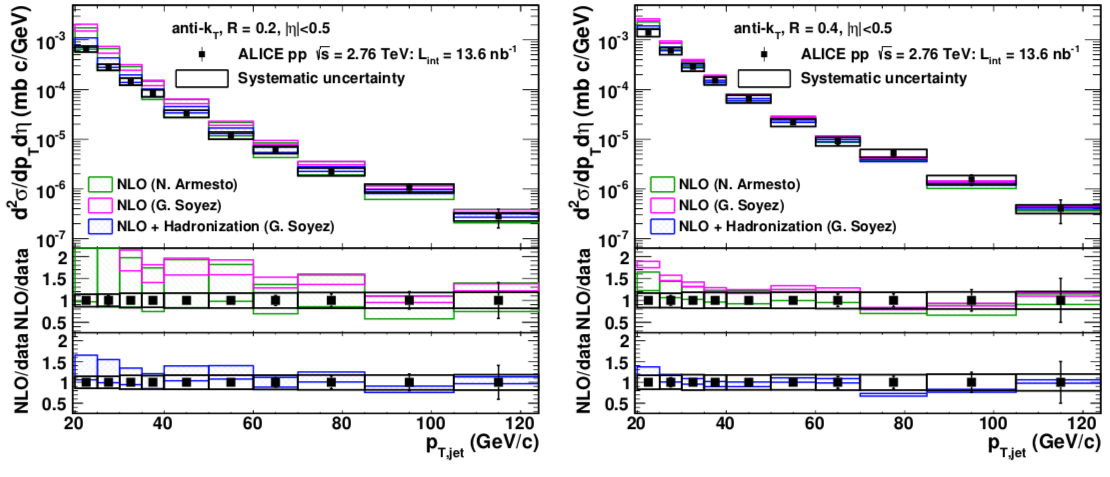
\includegraphics[width=17cm]{AliceppRongRong}
\centering
\caption{Inclusive differential cross section from the 2.76 TeV proton proton run with ALICE}
\label{fig:RunEff}
\end{figure}

\begin{figure}[h]
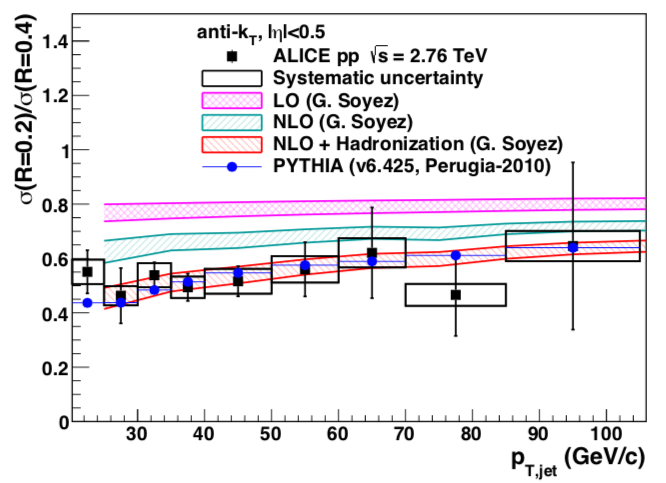
\includegraphics[width=10cm]{AliceRatioRongRong}
\centering
\caption{LHC state during the 8 TeV run. }
\label{fig:RunEff}
\end{figure}

\begin{figure}[!tbp]
  \centering
  \begin{minipage}[b]{0.4\textwidth}
    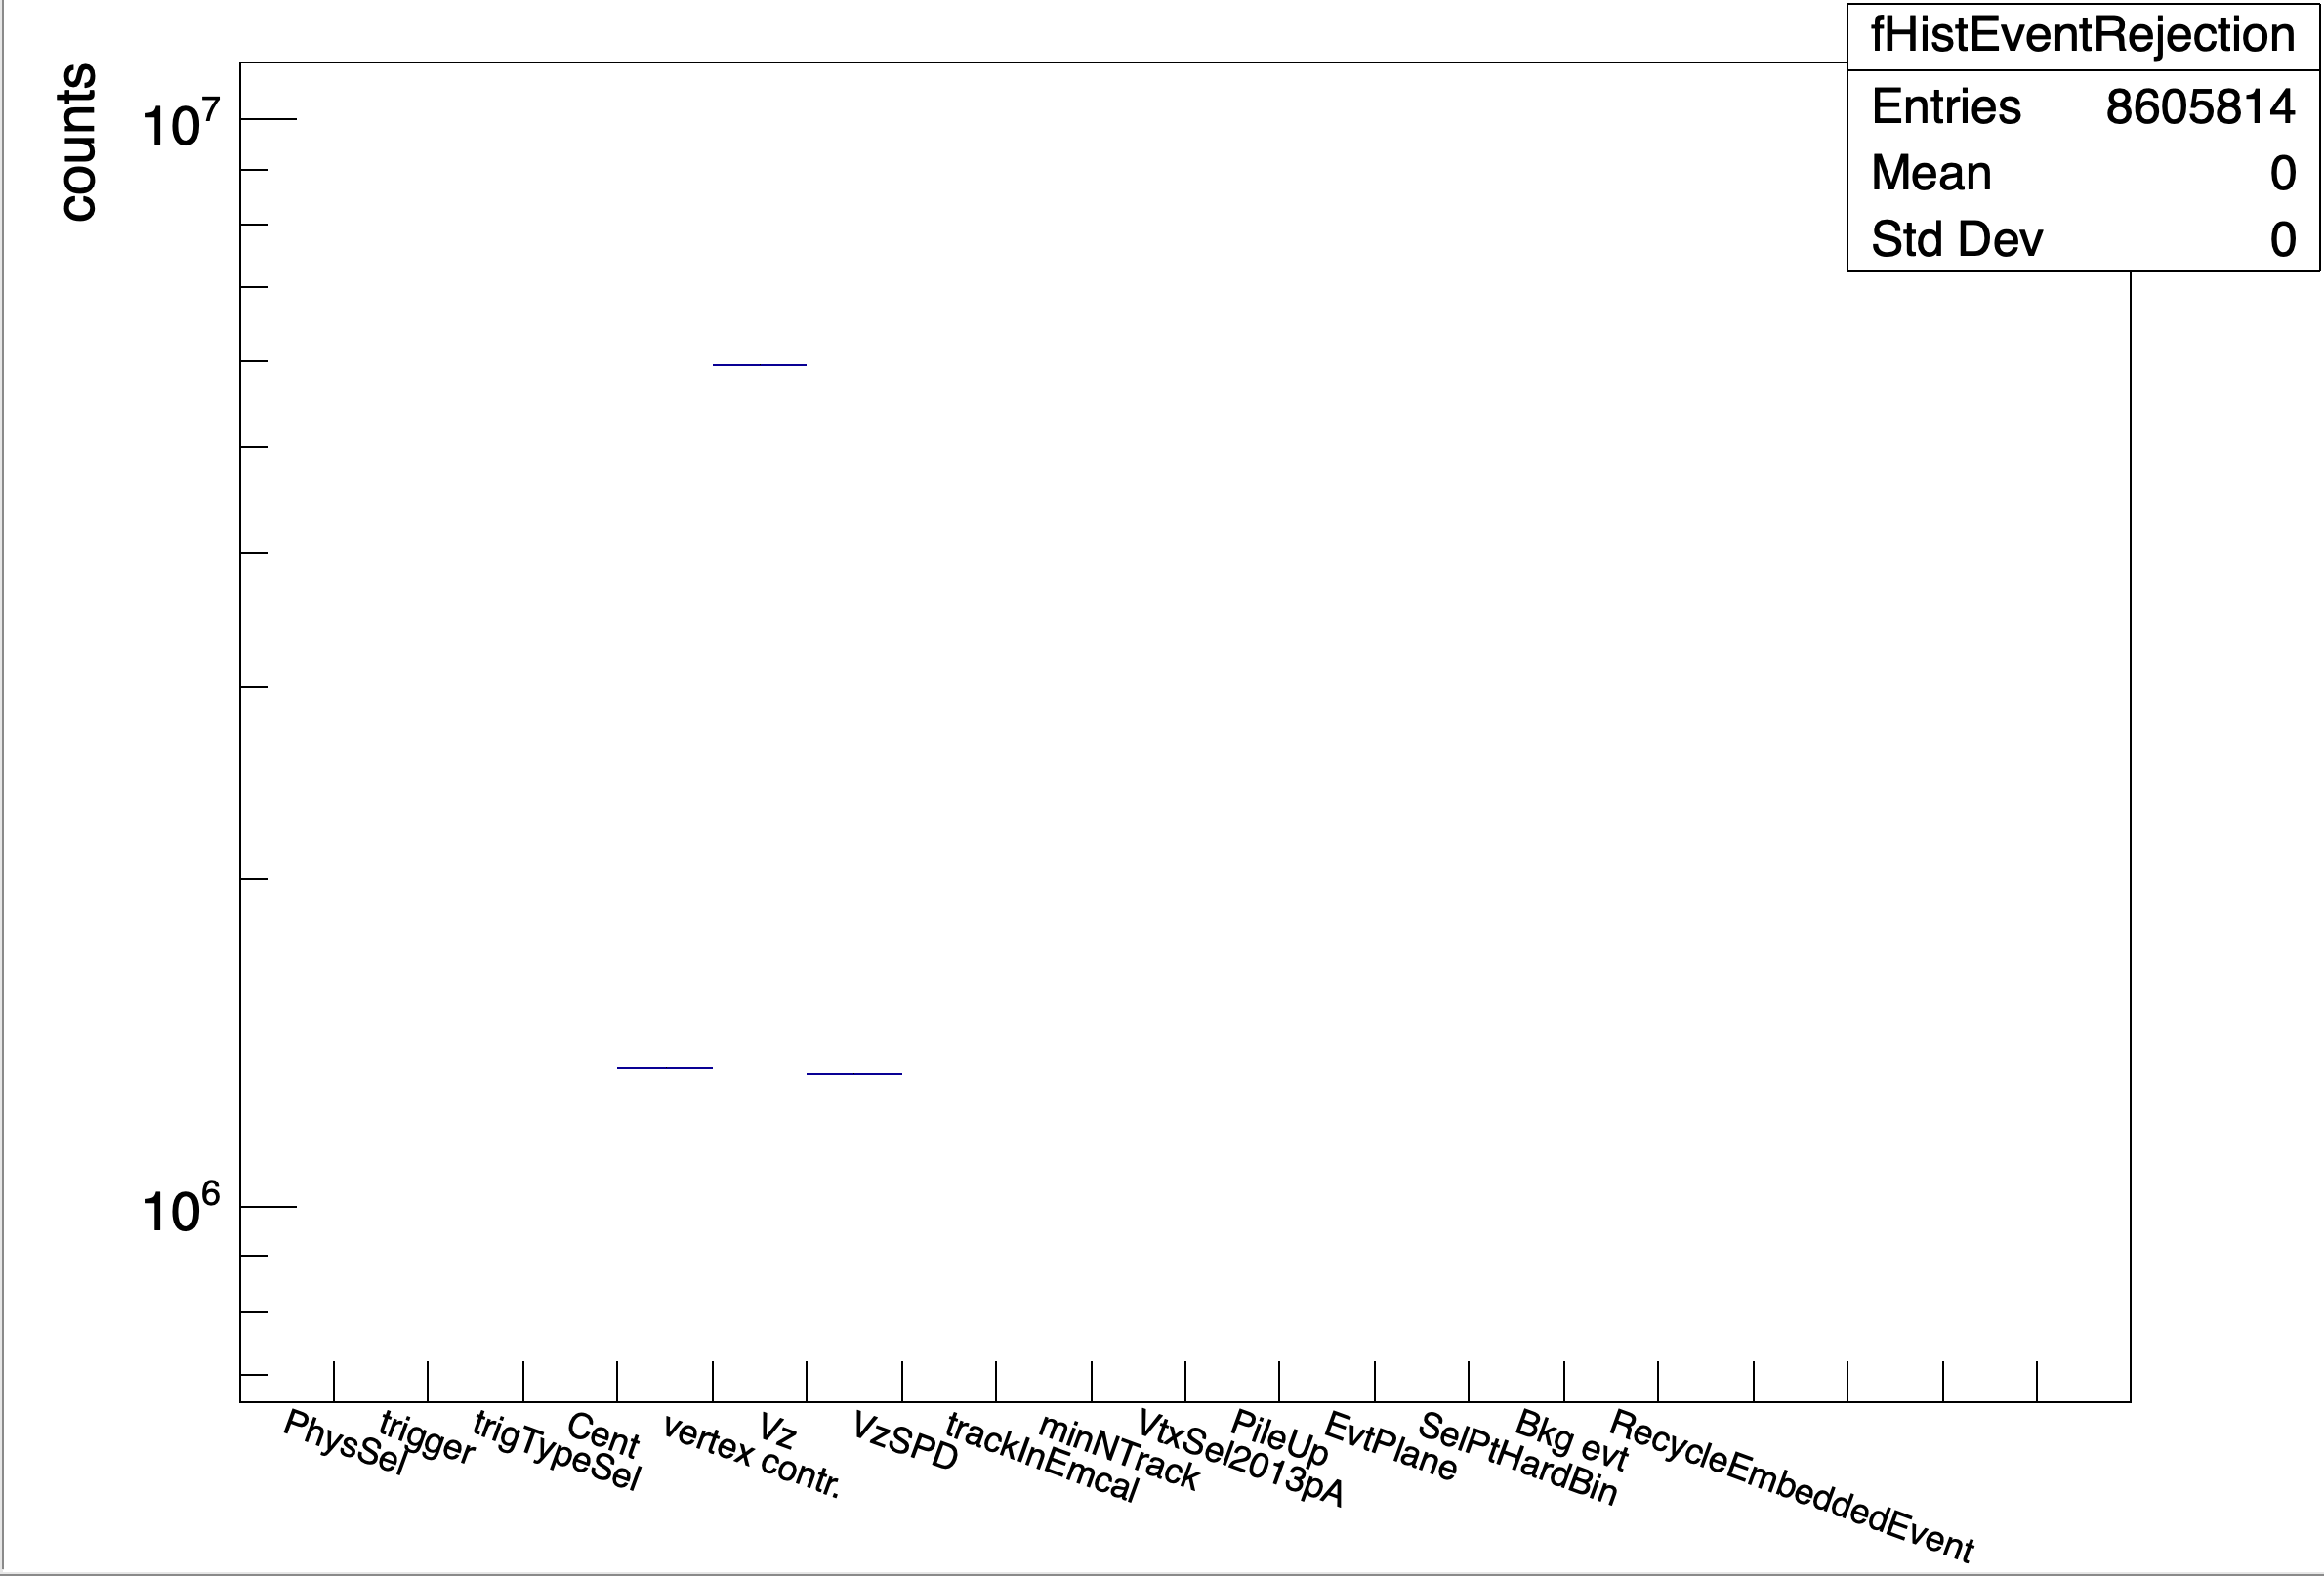
\includegraphics[width=\textwidth]{EventRejectionMB}
    \caption{Mimimmum Bias Event Rejection}
  \end{minipage}
  \hfill
  \begin{minipage}[b]{0.49\textwidth}
    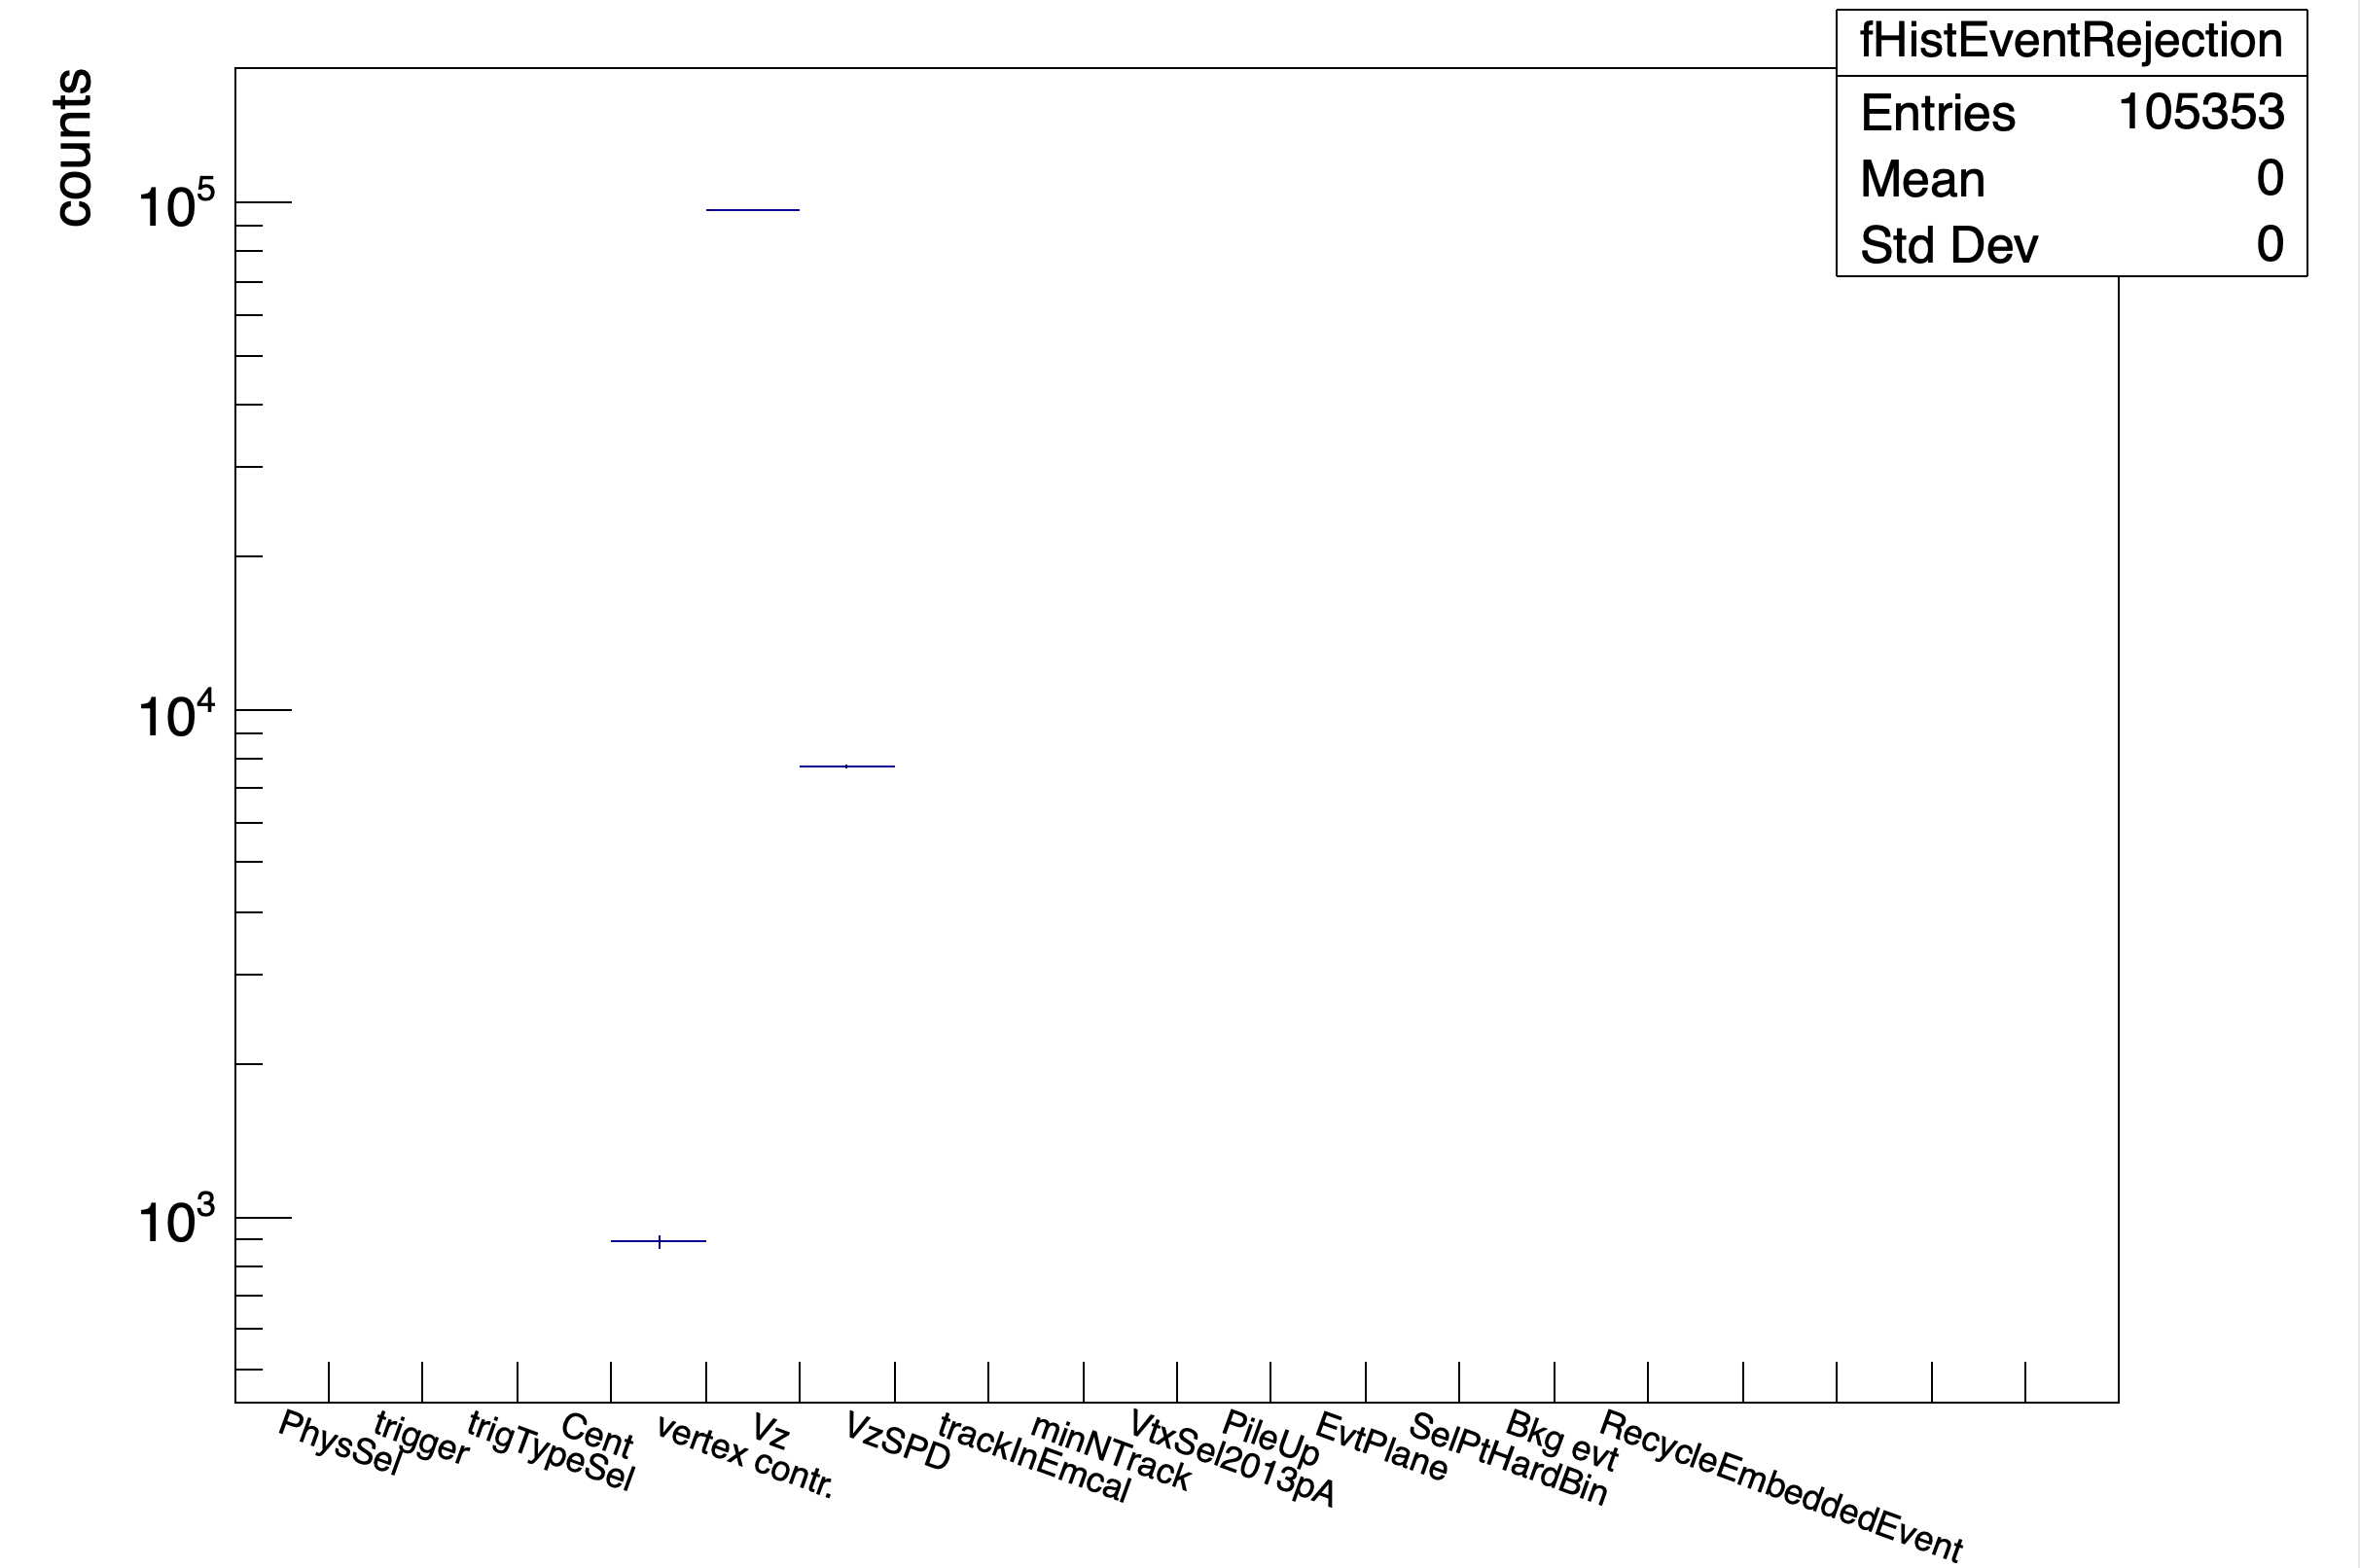
\includegraphics[width=\textwidth]{EventRejectionEGA}
    \caption{Emcal Triggered Event Rejection}
  \end{minipage}
\end{figure}

\fi

\section{Conclusion}

Jet cross-sections are a result of QCD interactions while the ratios of the cross-sections for jets of different radii probe the hadronization process.  The essentials nature of how hadronization effects the jet cross-sections is still an open question and should be probed in future measurements at the LHC.  ALICE is in the unique position of being able to reconstruct full jets over a wide kinematic range, especially to low momentum.  
This thesis presents the first measurements of inclusive full jets at $\sqrt{s} = \,$ 8 TeV using the ALICE detector.  It also presents the procedure by which using a set of corrections and QA criteria we may obtain results comparable to pQCD Monte Carlo simulations.  The agreement between the results and Monte Carlo simulations show the jets are a well calibrated probe.  In terms of the kinematics reach the results of this thesis are in good agreement with QCD calculations down to 20 GeV/c through 100 GeV/c in $p_{T}$.  This range may be extended with better Monte Carlos in the furture and this is currently being worked on until the results are published.  With a better Monte Carlo production we could see the range extend to between 5 GeV/c to about 200 GeV/c in $p_{T}$.  The comparisons with the Monte Carlos agree well with the most tension lying with PHOJET.  However, this results are expected to improve once an improved GEANT4 Monte Carlo that models the EMCal trigger is made available.  It is striking how well both hadronization models, the Lund-String model and Clusterization model encompassed by Pythia and Herwig agree with the data.  These are fundamentally different physics phenomenology and it begs the question to why this is?   It is interesting and exciting that some of the initial questions first posed when I started my Ph.D. work remain and I am hopefully for new insights from future work in both theory and experiment.  

The results from this thesis can also be used in future heavy-ion runs to probe jet quenching as these results would serve as a baseline comparison.  The work in this thesis also presents the first jet measurements from ALICE down to 10 GeV/c, which will be important for probing energy loss in the QGP.  By measuring these very low energy jets we can probe the full energy loss mechanism for partons traversing the QGP.  Previous higher energy jet results would tend to bias to jets that traveled a very short distance through the QGP.

With the increase in energy and luminosity seen at the LHC we have moved into the era of high-precision testing of pQCD.  The work set forward by this thesis sets the stage for using jets in the future at CERN, especially after the high luminosity upgrade of the LHC is complete.  Although it dates to 2012 the 8 TeV contains some of the largest data sets available at a given energy from the LHC.  This makes it an important data set and worthy of future investigations.  I'm proud of the work presented in this body, both in terms of the data analysis and engineering aspect.  What results we will gain from the upgraded LHC and jets is only left to our imagination and to nature's mercy.